\documentclass[12pt, a4paper, oneside]{article}\usepackage[]{graphicx}\usepackage[]{color}
%% maxwidth is the original width if it is less than linewidth
%% otherwise use linewidth (to make sure the graphics do not exceed the margin)
\makeatletter
\def\maxwidth{ %
  \ifdim\Gin@nat@width>\linewidth
    \linewidth
  \else
    \Gin@nat@width
  \fi
}
\makeatother

\definecolor{fgcolor}{rgb}{0.345, 0.345, 0.345}
\newcommand{\hlnum}[1]{\textcolor[rgb]{0.686,0.059,0.569}{#1}}%
\newcommand{\hlstr}[1]{\textcolor[rgb]{0.192,0.494,0.8}{#1}}%
\newcommand{\hlcom}[1]{\textcolor[rgb]{0.678,0.584,0.686}{\textit{#1}}}%
\newcommand{\hlopt}[1]{\textcolor[rgb]{0,0,0}{#1}}%
\newcommand{\hlstd}[1]{\textcolor[rgb]{0.345,0.345,0.345}{#1}}%
\newcommand{\hlkwa}[1]{\textcolor[rgb]{0.161,0.373,0.58}{\textbf{#1}}}%
\newcommand{\hlkwb}[1]{\textcolor[rgb]{0.69,0.353,0.396}{#1}}%
\newcommand{\hlkwc}[1]{\textcolor[rgb]{0.333,0.667,0.333}{#1}}%
\newcommand{\hlkwd}[1]{\textcolor[rgb]{0.737,0.353,0.396}{\textbf{#1}}}%

\usepackage{framed}
\makeatletter
\newenvironment{kframe}{%
 \def\at@end@of@kframe{}%
 \ifinner\ifhmode%
  \def\at@end@of@kframe{\end{minipage}}%
  \begin{minipage}{\columnwidth}%
 \fi\fi%
 \def\FrameCommand##1{\hskip\@totalleftmargin \hskip-\fboxsep
 \colorbox{shadecolor}{##1}\hskip-\fboxsep
     % There is no \\@totalrightmargin, so:
     \hskip-\linewidth \hskip-\@totalleftmargin \hskip\columnwidth}%
 \MakeFramed {\advance\hsize-\width
   \@totalleftmargin\z@ \linewidth\hsize
   \@setminipage}}%
 {\par\unskip\endMakeFramed%
 \at@end@of@kframe}
\makeatother

\definecolor{shadecolor}{rgb}{.97, .97, .97}
\definecolor{messagecolor}{rgb}{0, 0, 0}
\definecolor{warningcolor}{rgb}{1, 0, 1}
\definecolor{errorcolor}{rgb}{1, 0, 0}
\newenvironment{knitrout}{}{} % an empty environment to be redefined in TeX

\usepackage{alltt} % Paper size, default font size and one-sided paper
%\graphicspath{{./Figures/}} % Specifies the directory where pictures are stored
%\usepackage[dcucite]{harvard}
\usepackage{rotating}
\usepackage{amsmath}
\usepackage{setspace}
\usepackage{pdflscape}
\usepackage{appendix}
\usepackage[flushleft]{threeparttable}
\usepackage{multirow}
\usepackage[comma, sort&compress]{natbib}% Use the natbib reference package - read up on this to edit the reference style; if you want text (e.g. Smith et al., 2012) for the in-text references (instead of numbers), remove 'numbers' 
\usepackage{graphicx}
%\bibliographystyle{plainnat}
\bibliographystyle{agsm}
\usepackage[colorlinks = true, citecolor = blue, linkcolor = blue]{hyperref}
%\hypersetup{urlcolor=blue, colorlinks=true} % Colors hyperlinks in blue - change to black if annoying
%\renewcommand[\harvardurl]{URL: \url}
 \usepackage{listings}
  \usepackage{tikz}
 \usetikzlibrary{arrows,positioning}
 \usepackage{color}
 %\graphicspath{{../Pictures/}}
\definecolor{mygrey}{gray}{0.95}
\lstset{backgroundcolor=\color{mygrey}}
\IfFileExists{upquote.sty}{\usepackage{upquote}}{}
\begin{document}
\title{International Capital Flows and Speculation}
\author{Rob Hayward\footnote{University of Brighton Business School, Lewes Road, Brighton, BN2 4AT; Telephone 01273 642586.  rh49@brighton.ac.uk. }} 
\date{\today}
\maketitle
\begin{abstract}
The importance of gross international capital flows has become a more significant feature of the international financial system in the last 25 years.  As a result there has been increased attention paid to the nature of these flows and the effect that they have on the exchange rate and real economic activity.  This study seeks to augment portfolio flows with information about speculative activity to dientanble the portfolio adjustment from short-term activity.  A structural vector autorgressive model (SVAR) of these flows and the US real exchange rate indicates that shocks to speculative activity has real and persistent effects.   
\end{abstract}
\section*{Introduction}
Standard DSGE models can be opened up to the world to assess trade and exchange rates.  However, the nature of the model means that the main focus is the disturbance from equilibrium and the path back to stability.  These disturbances are stochastic and  not the main part of the analysis.\footnote{For an overview of the open economy models \citep{Obstfeld1995Redux} for a full treatment of the conventional DSGE models \citep{Woodford2003} and \citep{OandR}.}  One way to gain an understanding of the dynamics behind the disturbances to equilibrium is to leave the current account and to analyse the effect of capital flows on the real exchange rate.    The \emph{FIH} suggests that there will be significant and real macroeconomic effects from speculation.  The aim of this chapter is to understand more about the role of speculation on the real exchange rate and to see how far the addition of measures of speculative activity can add to the explanatory power of capital flow models of the exchange rate.    It is found that the addition of measures of speculative activity have real effects on the exchange rate and that these effects dominate those of net equity, bond and foreign direct investment, suggesting that speculation in the foreign exchange market is even more powerful and important than previously thought.  % Do we need something else here?   DSGE?  

Standard monetary and portfolio balance models of foreign exchange have been augmented with non-linear relationships and incorporate recent developments in the modelling of expectations as well as a deeper analysis of the nature of the distribution of asset price returns (see Chapters \ref{Chapter3} and \ref{Chapter4} for some examples of these techniques).  However, while the medium-to long-term direction of exchange rates can sometimes be projected with some confidence, short-term foreign exchange forecasting has been much less successful.  In the first decade of the twenty first century, the US dollar has defied a widening current account deficit which would, on a range of conventional theories,  be expected to cause a large depreciation.  Large capital inflows, drawn by a buoyant economy and then by the apparent safety and liquidity of US assets,  are usually cited as reasons for the resilience of the US unit.  However, the empirical support for this assertion remains fragile. 
 
This chapter seeks to get a fuller understanding of exchange rate dynamics by building a system to examine the interplay of exchange rates and capital flows.  A range of sources are used to construct series to measure the flow of international capital.   Vector Autogregression (VAR) is employed to deal with the issue of endogeneity with plausible and naive restrictions identifying the effect that shocks to a variety of different forms of capital flow have on the real exchange rate.   Understanding more about the relationship between capital flows and real exchange rate is important in a world where these financial account activities are becoming increasingly significant and where persistent current account imbalances have been seen to have major global consequences\footnote{There is a strand of thought that sees the global imbalance as one of the main causes of the recent financial crisis.  This view argues that the US current account deficit required a balancing inflow of capital to the US and that this capital flow either reduced long-term interest rates or removed a portion of safe assets from the market, as central banks bought safe and liquid treasuries.  The first of these reduced US long-term interest rates,combining with the Fed's easy policy to make house purchase more attractive.  The second encouraged the creation of synthetic 'safe' assets like the most credit-worthy tranches of CDOs and other financial innovations which increase the amount of credit in the US economy \citep{Eichengreen2006Global}, \citep{Obstfeld2009Global}, \citep{Portes2009Global} and others.} as well as more usual effects of real exchange rate misalignment can have on domestic economies\footnote{\label{note1}From Keynes' Economic Consequences of Mr. Churchill \citep{Keynes1925Churchill} through to current debate about competitiveness in the euro area, the level of the real exchange rate has been widely regarded as an important determinant of domestic economic conditions.  For a discussion of the issues that would determine the appropriate level for CEE and CIS countries to join the Euro \citep{Jens}.}.  This paper takes the US as its focus for three reasons:  there is a large amount of public data available about the international sale and purchase of US financial assets which can help to overcome the paucity of information that has been something of a constraint on testing of comprehensive capital flow models; the US represents a most significant example of the divergence between conventional theory and the evolution of exchange rates;  the US is at the heart of the global imbalance story.  

The main findings of the research are that capital flows associated with relative interest rates and speculative sentiment have significant effects on the level of the real exchange rate.  Net equity flows also appear to be positively related to the real exchange rate but the picture with net foreign direct investment and net bond flows is more ambiguous.  When bond flows are divided into those conducted by official organisations (like central banks) and others, the former have the expected positive effect, because they reflect central bank foreign exchange intervention, while the latter do not seem to be influential. The rest of this chapter proceeds as follows: section two reviews the literature; section three discusses methodological issues; section four presents the results; section five concludes. 
  
\section{Literature review}
There are two broad strands to the way that exchange rates are to be understood:  a focus on real goods and services and the current account, and a focus on capital flows and the financial account.\footnote{Throughout this work, the term 'financial account' will refer to the mirror of the current account of the balance of payments recording the main portfolio or real investment flows that take place between the home countries and the rest of the world.  This is consistent with the terminology used by the International Monetary Fund \citep[ch.2 p. 9]{IMFBOP}.  The term 'capital account', which is used for these activities in some places, is here reserved for valuation adjustments to holding of international assets and will not play a significant part in the story.} The former is based on the law of one price with the theory of purchasing power parity implying that exchange rates will adjust to ensure that price levels in different currencies will be broadly similar.  The latter seeks to understand the international flows of capital, usually by looking at international investors response to relative rates of return of different assets in different currencies.  

\subsection{Purchasing power parity}  
Gustav Cassel is credited with the first use of the term \emph{purchasing power parity} as the ``quotient between the purchasing power of money in one country and the other'' \citep[p.298]{Cassel1916Present}.  

The average price of a basket of home goods and services is represented by $P$, those of another country by $P^*$, with the * superscript used throughout to represent overseas variables, and the exchange rate expressed as domestic currency per unit of overseas as $S$, if arbitrage is possible, the law of one price implies that price level of the domestic basket should be the same as the overseas basket. 

\begin{equation}
 P^*S=P
\end{equation}

or, using lower case to denote logarithms and re-arranging,

\begin{equation}
\label{eqref:ppp}
s = ln(S) = lnP - lnP^* = p-p^*
\end{equation}

Therefore, under PPP, the exchange rate should adjust to ensure that if prices in one country change, there is a potential arbitrage that will tend to bring them back into line.  The adjustment may come through the price via the effect of changes in demand at home and abroad or it may come through the exchange rate, if that is allowed to fluctuate, due to demand for currency used to satisfy purchase of relatively cheap products and services.   This may be called \emph{absolute PPP} while a less strict version of \emph{relative PPP} would imply that changes in relative price level or two countries will tend to equalise.

\begin{equation}\label{relPPP}
\Delta S=\frac{\Delta P}{\Delta P^*}
\end{equation}

The real exchange rate (Z)  is then the relative price of a representative basket of goods and services when domestic prices have been converted into a common unit.   

\begin{subequations}
\begin{align}
Z=\frac{SP^*}{P}
\end{align}
so, in logs
\begin{align}
z = s + P^* - p
\end{align}
\end{subequations}

where $z$ is the real exchange rate. Given two countries, an appreciation of the real exchange rate for the home country (a decrease in Z) means that its relative money prices have risen compared to the overseas country.  The theory of PPP says that the real exchange rate should be stable or that is should return to a long-run level. Therefore the test of the theory of  PPP is that the real exchange rate is stable, mean-reverting or stationary.\footnote{A stationary series is one that has, amongst other things, an arithmetic mean that is stable over time.   Therefore, statistical tests of stationarity, such as unit root tests,  have been used to test the PPP proposition.  These tests have been less conclusive than would be anticipated.  For more details about the issues associated with the statistical power of the tests of stationarity and the methods that have been used to try to overcome them \citep{TaylorPPP}.  One of these is the apparent positive relationship between the real exchange rate and the level of economic development or GDP per capita.  The Harod-Belassa-Samuelson theory is discussed more fully in Section \ref{secref:HBS}} 

\subsection{Uncovered interest parity}
\label{secref:UIP}
The forward rate is the rate that is set now for an exchange of currencies in the future.  Covered Interest Parity (CIP) asserts that, given the free flow of international capital and competitive markets,  the difference between the spot rate and the forward rate must be equal to the interest rate differential for the two currencies for the same period.  Otherwise, there is an arbitrage opportunity that will encourage parity to be restored.  

\begin{equation}
\frac{F_{t, j}}{S_t} \times (1 + i_{t,j}^*) = (1 + i_{t,j})  
\end{equation}

%should I use I rather than i (which could be for logs)?
where $F_{t, j}$ is the forward exchange rate at time t for domestic currency in terms of overseas for j periods ahead;  $S_t$ is spot exchange rate under the same terms at time t; $i_{t,j}$ is the interest rate for the home currency in period t for j periods ahead; $i_{t, j}^*$ is the interest rate for the overseas currency at time t for j periods ahead.

Therefore, 

\begin{equation}
\frac{F_{t,j}}{S_t} = \frac{(1 + i_{t, j})}{(1 + i_{t, j}^*)} 
\end{equation}

 Re-arranging

\begin{equation}
\label{eq:fw}
\frac{F_{t,j} - S_t}{S_t} = \frac{(i_{t,j} - i_{t,j}^*)}{(1 + i_{t,j}^*)} 
 \end{equation}

%we will have to add the reference to Muth here at some point. 
If it is assumed that expectations are formed rationally (see Section \ref{secref:noise} on speculation, information and expectations for a fuller discussion of rational expectations and Section \ref{secref:ex} below for an assessment of what happens when this assumption is relaxed), the forward rate should be the best, unbiased estimate of the future spot rate and therefore, Equation \ref{eq:fw} becomes.  

\begin{equation}
\frac{E[S_{t+j}] - S_t}{S_t} = \frac{(i_{t, j} - i_{t, j}^*)}{(1 + i_{t, j}^*)}
\label{eq:UIP}
\end{equation} 

if $i^*$ is relatively small, this can be approximated by 

\begin{equation}
E[s_{t+j}] - s_t = i_{t,j} - i_{t,j}^* 
\end{equation} 

where $s_t$ is the log of the exchange rate at time t, $s_{t + j}$ is the log of the exchange rate at t plus j, $i_{t, j}$ is the j-period interest rate at time t and $^*i_{t, j}$ is the the foreign currency j-period interest rate at time t.  

Assuming that CIP holds so that the forward rate can account for the interest rate differential, a test of UIP can take the form of 

\begin{equation}
\label{eq:uip}
\Delta s_{t + j} = \beta_0 +\beta_1 f_{t+j} + \varepsilon
\end{equation} 

where $\Delta s_{t + j}$ is the change in the log of the exchange rate between period t and j, $f_{t+j}$ is the forward premium expressed as the difference between the logs of the spot rate and the forward rate for period j; $\varepsilon$ is an error term that is assumed to be an independent and identically distributed random variable with a mean of zero, while $\beta_0$ and $\beta_1$ are the coefficients to be estimated.  If UIP holds, $\beta_0$ should be equal to zero and $\beta_1$ should be equal to unity as the forward rate should be an unbiased estimate of the future exchange rate.   There may be frequent errors in the estimate (represented by $\varepsilon$), but these should on average be zero. 

However, this standard test of UIP consistently finds that estimates of  $\beta_1$ are less than one.  A meta-study by Froot and Thaler found that the average of 75 published estimates had an average value of -0.88 for $\beta_1$ \citep*{FrootUIP}.   This is sometimes called the \emph{forward premium puzzle}.  Hodrick gives  a thorough overview of the evidence on unbiasedness \citep{Hodrick1988}.  
%need further and more recent evidence here.  

\subsection{Monetary approaches}
\label{secref:money}
To get a fuller understanding of the relationship between the exchange rate and other parts of the economy, economists have sought to augment the theory of PPP by adding theories for money and expectations.   Given the \emph{quantity theory of money}, which states that, assuming stable money demand and exogenous money supply, the price level is function of the quantity of money, thus PPP is determined by the growth of relative money supplies.       Expectations can start to play a role as relatively high money growth can create an instant anticipation that the exchange rate will adjust with a depreciation as relatively high money growth leads to an anticipated increase in relative prices, even if prices are sticky and adjustment takes some time. Therefore, there are two broad monetary models: the flexible price and sticky price models.  The first of these will assume that PPP always holds.  See, for example \citep{Frenkel1976Money},  \citep{Mussa1976Money} and \citep{Bilson1978Money}.  Here, the nominal exchange rate $(s)$ is a function of relative prices, as in Equation \ref{eqref:ppp}, 
while the price level is determined by conditions in the money market at home

\begin{equation}\label{moneyhome}
m-p=\alpha y + \beta i 
\end{equation}

and abroad, assuming that domestic and overseas money demand functions equivalent. 

\begin{equation}\label{moneyaway}
m^*-p^*=\alpha y^* + \beta i^{*}
\end{equation}

Everything is in logs; $m$ is the stock of money, $p$ is the price level, $y$ is national income and $i$ is the nominal interest rate or, more appropriately, $m$, $p$ and $y$ are deviations from their long-run growth path, $\alpha$ and $\beta$ are parameters to be estimated for the income elasticity of money demand and the price elasticity of money demand measured by the interest rate opportunity cost.  Plugging these Equations \eqref{moneyhome} and \eqref{moneyaway} into the exchange rate Equation \eqref{eqref:ppp} gives

\begin{equation}
s=(m-m^*)-\alpha (y-y^*) - \beta(i-i^*)
\end{equation}

To the extent that relatively high money growth is not a function of an increase in relative money demand (as a consequence of a change in income or the opportunity cost of money), there is an effect on the exchange rate via price levels and the law of one price.  

However, prices do not instantly adjust to changes in the stock of money.  With flexible exchange rates it is clear that there is a gap between the swift adjustment of exchange rates in the asset market and the more gradual adjustment of goods prices.  Therefore, the sticky price model of exchange rates is more widely known and more defensible against the empirical evidence of sluggish adjustment of prices to economic shocks (including monetary shocks).  This model also allows some integration of the two strands of exchange rate analysis as what is happening in the goods markets is combined with what is happening in the asset market.  One of the pioneering examples of the sticky price approach is the Dornbusch Overshooting model \citep{Dornbusch1976Expectations}. 

The key to this model is the gap between the gradual adjustment of prices in the goods market and the more rapid change for asset market prices.  PPP does not always hold as there are short-run deviations as relative prices adjust to the relative growth of money stocks.  The model is augmented with uncovered interest parity (UIP) condition to make a connection to the asset markets.  

\begin{equation}\label{UIP}
E[\Delta s_{t+1}|\Omega_t]=\beta(i-i^*)
\end{equation}

Where $E$ is the expectations operator, $\Delta s_{t+1}$ is the change in the exchange rate between $t$ and $t + 1$ and $\Omega_t$ is the information set available at time $t$.  Then, given the level of prices and the interest rate differential, there is a long-run level for the exchange rate and a current spot rate that matches the interest rate differential. 

\begin{equation} 
s=(m-m^*)-\alpha(y-y^*)-E[\Delta s_{t+1}|\Omega_t]
\end{equation}

A permanent increase in nominal quantity of money will lead to an instant adjustment of the exchange rate which is a reflection of the long-run change in the relative price level and the short-run change in relative interest rates.  There is over-shooting here because for any given price level, the exchange rate adjusts instantly to clear the asset market.  In the case of a monetary expansion that will eventually lead to higher prices and a fall in the nominal exchange rate, there is overshooting of the exchange rate to maintain equilibrium in the asset market as money growth will also reduce the domestic interest rate relative to other countries and this requires an appreciation of the nominal exchange rate to compensate for the income loss, as demanded by the model's assumption of UIP.  While the overshooting model helped to explain the volatility of floating exchange rates and is consistent with the evidence of a positive relationship between interest rates and the exchange rate, the implication that overshooting would be followed by a gradual adjustment back to the appropriate PPP level does not appear to be supported (see Chapter \ref{Chapter4} Section \ref{secref:UIP2} for a fuller discussion of this, including speculative attempts to take advantage of this failure).    

\subsection{Harrod-Balassa-Samuelson}\label{secref:HBS}
PPP occupies a central position in international economics and has acquired a number of extensions in the face of some discomforting empirical evidence \citep{TaylorPPP}.   Real exchange rates are stationary in many cases but there are also times when there appear to be deterministic trends \citep{Froot1995Purchasing}.  Tests on the stationarity of the real rate is very sensitive to the period studied and the existence of financial crises \citep{ZhouKutanPPP}.  For an an overview of empirical evidence \citep{Taylor2004Purchasing}.    The law of one price may hold for commodities which are traded and exchanged around the world.  However, while the price of some traded goods may be very similar in different countries, transaction costs, taxation or other frictions or barriers for many products and services very often start to drive a wedge between prices in different countries.  Though  Krugman  finds that PPP generally holds in the long-run despite significant short-run deviations, there is a tendency for the real exchange rate to appreciate with economic development \citep{Krugman1978PPP}.  
%There are a lot of goods and services that are not easily arbitraged.  Non-traded good may be unaffected by international competition and prices.  If sheltered non-traded goods tend to be more service-orientated, the scope for productivity improvement may not be present.  Then, for a consumption basket that is made up in one part of a manufacturing traded good and one part of a non-traded service good, the improvement in productivity in the manufacturing sector will allow wages to increase without an equal increase in unit labour costs or prices while, assuming a labour market that is not segmented, the wage rise will tend to spill over to prices in the non-traded service sector where productivity has not improved.   This will raise the price of non-traded service goods relative to traded manufacturing goods and will push up a real exchange rate measured on a basket of traded and non-traded.  This will lead to an appreciation of the real exchange rate if it is measured as a basket of traded and non-traded goods.  


Harrod outlined the main ideas of what has come to be known as \emph{Harrod-Ballasa-Saumuelson Effect} in some of the early editions of his \emph{International Economics} textbook \citep{Harrod1933International}.  Balassa identified the evidence of a positive relationship between the per capita income levels and the real exchange rate with the explanation that productivity gains were mostly concentrated in the traded goods sector and that wage competition between traded and non-traded sectors would push up the relative price of non-tradables with development.  He supported this assertion with information about the productivity levels in different sectors of the economy of major nations and the relationship between the ratio of the GNP deflator to manufacturing wholesale prices to manufacturing per capita output  \citep{Balassa1964PPP}.  

This is the international outcome of \emph{Baumol's Effect} \citep{Baumol1966Performing} whereby the wages of those sectors of the economy that do not achieve productivity increases rise in some proportion to those sectors that do so as to maintain some equilibrium in the two sectors.   Baumol used the example of musicians playing a string quartet as an industry where productivity has not increased but where wages have risen in line with others in the economy.   De Gregorio conducted an analysis of sectoral price data for OECD countries in the period 1970 to 1985 and found that inflation in non-tradables exceeded that of tradables.  The investigation also found that a combination of a demand shift towards non-tradables and a faster pace of productivity growth in the traded goods sector were the main cause of this phenomenon \citep{DeGregorio1994International}. 


Samuelson argues that the frequent and prolonged deviations from purchasing power parity that are seen are a result of the wide spectrum of goods where unit labour requirements can differ in different countries  \citep{samuelson1964trade}.  Using the * for overseas variables, $a_i$ for the unit labour requirement for good $i$ (as Samulelson did), $(w)$ for money wages and $(s)$ for the exchange rate measured as the foreign price of domestic currency, it is possible to project two extremes between which the economy would move from a position of competitive advantage for all goods to a competitive disadvantage for all goods. 

\begin{equation}\label{samuelson}
Min\frac{a_i}{a_i^*} \leq \frac{w}{sw^*} \leq Max\frac{a_i}{a_i^*}
\end{equation}

Productivity differentials ($a_i/a^*_i$) define the boundaries for wage costs once they are translated into a common currency.  For example, if the most extreme productivity differentials are $1/5$ this means that the exchange rate adjusted wage differential cannot go above $1/5$ before all goods are uncompetitive; if $8/1$ is the maximum productivity extreme, the barrier is $8/1$ before all goods are competitive for the home country.  Within this range, for a given exchange rate, there is a borderline product where cost of production at home or abroad will be very similar, such that 

\begin{equation}
s=\frac{w}{w*}\frac{a_i}{a_i^*}
\end{equation}

The exchange rate can fluctuate between the two extremes and there will be a trade surplus or trade deficit depending on what part of the productivity spectrum the exchange rate occupies at one particular time. 

\begin{equation}
\frac{w}{w^*} Min \left [\frac{a_i}{a^*_i} \right ]\leq s \leq \frac{w}{w^*}Max \left [ \frac{a_i}{a^*_i} \right ]
\end{equation}

The price of most goods and services will not be in equilibrium and the borderline good will change over time in response to changes in productivity, preferences and demand - as well as the exchange rate. Therefore, the relative price of most goods in two countries will be different and the real exchange rate can fluctuate substantially over time.  This is before capital flows are allowed to have some effect.  Samuelson  states that ``once we leave barter equilibrium aside and admit capital movements and gold flows into the picture, the sky becomes the limit'' for the real exchange rate \citep[p. 146]{samuelson1964trade}. 

\subsection{The PPP adjustment process}
It should be no surprise, therefore, that the real exchange rate can fluctuate substantially.  Even when there is a return to a mean PPP value, it appears that this can take a considerable amount of time.  It has been common to assess the adjustment by measuring the so-called {half-life} of the deviation process.  This is the time that the exchange rate takes to return half way to PPP level after a shock (see \citep{Frankel1986} and \citep{FrankelFroot1987}).  In the most well known investigation of the speed at which the real exchange rate returns to parity after a shock,  Rogoff found that it would take an average three to five years for the real exchange rate to move half-way back to its original position after a shock \citep{RogoffJournal}.   This leaves a wide window where factors other than relative price can have a major influence on exchange rates.  

There are many historic examples where a significant deviation from PPP has been sustained for a considerable period.  In the Samuelson formulation, if there is one commodity for which there is comparative advantage, there can be others which become uncompetitive.  This deviation can be the result of having an endowment of one or more important commodities, goods or even services.  The \emph{Dutch Disease},\footnote{The Dutch Disease is the term coined by \emph{The Economist} for the experience of the Netherlands in the 1960s where discovery of large natural gas fields led to an increase in the trade surplus and some inflow of capital with a consequent appreciation of the real exchange rate to the point where the rest of the Dutch manufacturing sector became uncompetitive.  It is partly this experience which led the Norwegian government to create the Strategic Petroleum fund to hold receipts from Norwegian international crude oil sales in foreign currency to prevent real appreciation of the Norwegian Crown.  For a more formal overview of the Dutch Disease see \citep{CordenNeary}. Bruno and Sachs present a model of ``perfect foresight, intertemporal equilibrium''  that is used to analyse the effect that the discovery of north sea oil has on the UK economy \citep[p. 846]{SachsDutch}.} where the real exchange rate and wage rates are elevated to a point where much of the output of an economy is internationally uncompetitive, is an extreme example of this.  Though the appreciation of the real exchange rate in the Netherlands in the 1970s is the most usual example of this, the idea can also be more widely applied to cases like the UK where the presence of an international financial centre cause real exchange rate appreciation or the US where the production of safe and liquid international assets may also have the same effect.  In each case, there is evidence of this demand for assets having a substantial effect on capital flows that can lead a to sustained and significant effect on the real exchange rate.  
  
\subsection{International capital markets}
As a consequence of the rising prominence of international capital flows and as one response to the evidence of large and persistent deviations from PPP, there has been increased attention paid to the role of capital flows in determining  changes in the exchange rates.  To assess capital flows it is necessary to go back to the balance of payments and look at the relationship between trade and finance.  The standard model of international accounting defines the current account of the balance of payments as   

\begin{equation}\label{currentaccount} 
CA_1=B_{t+1}-B_t=Y_t+r_tB_t-C_t-G_t-I_t 
\end{equation} 

\citep[p. 15]{OandR}
where $B_{t+1}$ is the value of net foreign assets at the end of the current period, $Y_t$ is current income, $G_t$ is government spending in the current period, $I_t$ is domestic gross fixed capital formation and $CA_t=B_{t+1}-B_t$ is the balance of payments, stating that the current account must be financed or, in other words, offset by an equal change in the financial account.  The return earned on the net foreign assets held in the previous period is $r_tB_t$, with $r_t$ as the weighted average return on international assets.  If national savings is defined as national income less spending of households and the government, and denoted as $S_t$ \footnote{This is a little confusing given that $S_t$ has already been used to denote the nominal exchange rate.  However, given the convention in this area and in the absence of any clear, logical alternative, it will be followed for the next few paragraphs.} 

\begin{equation} 
S_t \equiv Y_t+r_tB_{t+1}-C_t-G_t 
\end{equation}

Equation \eqref{currentaccount} becomes

\begin{equation}\label{SI} 
CA_t=S_t-I_t 
\end{equation}  

or the current account balance is equal to the difference between domestic savings and investment. 
Therefore, in the absence of a government, the accumulation of net foreign assets will be equal to domestic savings less investment,  

\begin{equation}
 B_{t+1}-B_{t}=S_t-I_t
\end{equation} 

and the determination of the current and financial account becomes an issue of inter-temporal allocation of spending.  

To use this simple model of the balance of payments to assess more than one country and the exchange rate, the variables for an overseas country can be denoted with a superscript asterisk (*) as usual.   Therefore, $Y^*$ would be other-country income, $S^*$ would be other-country savings and $C^*$ denotes other country consumption.  Using the identity for income and output and allowing the two countries to trade goods and assets, would mean that 

 \begin{equation} 
Y_t+Y^*_t=(C_t+C^*_t) + (G_t +G^*_t)+(I_t +I^*_t) 
\end{equation}

The standard forward-looking representative agent used in these models would seek to smooth consumption over time and would therefore adjust savings and consumption to maximise utility in each period given expectations about future income and evolving preferences.\footnote{This smoothing can take place in a closed economy only if agents have heterogeneous endowments, preferences or expectations.  The idea is the same here, but the heterogeneity is across countries.}  Given the assumptions of this model, an increase in productivity and expected future income should lead to a current account deficit as the representative household takes advantage of a rise in the present value of future income.  The rundown in net foreign assets is compensated by the increased net present value of future income.  Obstfeld and Rogoff present a model of permanent balance of payment components based on an annuity value at the current interest rate to give a \emph{fundamental equation for the current account} \citep[p. 74]{OandR}.
Sachs provides one of the first of these long-run, dynamic, intertemporal models of current account (and therefore financial account) adjustment \citep{SachsCA}.  

\begin{equation} 
CA_t=B_{t+1}+B_t=(Y_t-\bar{Y})+(I_t-\bar{I})-(G_t-\bar{G}) 
\end{equation} 

where $\bar{Y}$, $\bar{I}$ and $\bar{G}$ are the \emph{permanent} levels of income, investment and government spending respectively based on discounting expected future values back to the present. For a constant interest rate, the permanent level of each component at time t is given by   

 \begin{equation} 
E[\bar{Y}]=\frac{r}{1+r}\sum_{t=s}^{t=\infty}\left (\frac{1}{1+r}\right)^{s-t}Y_s 
\end{equation}

This is an annuity of the component at the set interest rate.  This can be solved as infinite-period version of the standard two-period utility optimisation subject to budget constraints.\footnote{As such, this is a version of Friedman's \emph{permanent income theory} \citep{FriedmanConsumption}.  In the simple case where the representative agent's time preference (denoted $\beta$) is $1/(1+r)$, there is no government (G) or business activity (I) and output is exogenous and set a constant level $\bar{Y}$, the optimal consumption will be $C = \bar{C} =rB + Y$.  As simplifying assumptions are relaxed, the calculation becomes more complex, but the basic idea remains the same: any change in expectations about future output, spending or interest rates results in an adjustment of inter-temporal consumption through the current account and, therefore, the financial account \citep[pp. 59-89]{OandR}.}    This implies that current account imbalances are the result of changes in expected long-run levels of income, investment or government spending and the rate of interest or preferences.   The model suggests that if the capital accumulation required for economic development cannot be satisfied by domestic savings, the imbalance of savings and investment require a current account deficit or a financial account surplus and a run-down of net foreign assets, balanced by an increase in expected future income. 

When the other parts of the conventional new-Keynesian macroeconomic model are added, this is the basis for the open economy dynamic stochastic general equilibrium model.  Again, see \citep{Obstfeld1995Redux} for a comprehensive overview of the main features of the model and \citep{Lane2001} for a survey of the different varieties of open-economy DSGE model. 

However, as is the case with the more general criticism of DSGE models, when the model is opened up to the rest of the world (and called an open-economy dynamic general equilibrium model), equilibrium is assumed and the main focus therefore is to assess the way back to the equilibrium once at shock has created a disturbance.  The, perhaps more interesting, cause of the shocks or the immediate consequences of the shocks are largely ignored.  For the exchange rate, the anchor is the path of relative money growth and relative consumption demand at home and abroad.  As a result of a money, preference or productivity shock, the exchange rate jumps immediately to the new trajectory that is consistent with equilibrium, prices may adjust in a sticky fashion, but there is no scope for deviations from the short-run path back to equilibrium.  As indicated in the footnotes, Obstfeld and Rogoff ``are assuming away speculative exchange rate bubbles'' \citep[p 640]{Obstfeld1995Redux}.  In addition, the models usually assume that representative households are risk averse and fully diversified, leaving no unsystematic risk.  To get to an analysis of the short-term capital flows that can affect the exchange rate outside of the equilibrium, it is necessary to make the models increasingly complex\footnote{See \citep{Devereux2011Portfolio} for an example of an attempt to apply portfolio optimisation to the international financial economics.  The big difficulty is that optimisation weights have to be constructed but, in turn, portfolio weights will determine the return on international assets.  Devereux and Southerland find a complex solution to this as one way of understanding international asset allocation.  However, it is not clear that this method would be able to deal with short-run disturbances and exchange rate shocks.} %need a reference for these DSGE models with additions
or to break away from general equilibrium to focus on individual parts of the economy.  To understand how international demand for assets can drive exchange rates general equilibrium, representative agents and long-run expectations about income and productivity must be abandoned. To examine the relationship between short-term capital flows and the exchange rate it is necessary to put capital flows back to the centre of the analysis. 
 
\subsection{Portfolio flows}
To focus exchange rate models on capital flows is not entirely new.  Portfolio balance models have been around since at least the 1970s.  Amongst those that have contributed to this research are \citep{Kouri1974International} \citep{Kouri1977}, and \citep{Branson1985International}.  % these references need to be completed

%here are some up-to-date references. 
%http://www.econbrowser.com/archives/2008/07/disorderly_adju.html
%http://www.econbrowser.com/archives/2008/09/implications_of.html

Portfolio balance models can look at either stocks of international assets or the flow of funds into international assets.   The major problem that the early versions of these models encountered was the lack of data against which they could be evaluated.   Information about the flow of capital has traditionally been very difficult to collect.  As a result the early models tended to simplify capital flows. The first of the models would only include international bonds $B$ as being representative of broader asset markets and the supply of bonds was frequently measured as the accumulation of government debt.   This is a two country model. 

\begin{equation} 
B_f=\beta W_d
\end{equation}

Where $B_d$ are domestic bonds and $B_f$ are foreign bonds as denoted by the sub-script.  $\beta$ is the share of domestic wealth (denoted $W_d$) that is allocated to overseas bonds.    For these models, it is  assumed that the share of $B_f$ would be determined by rates of return, relative interest rates and expected changes in the exchange rate\citep{Kouri1974International}.  Indeed, this can be seen as a portfolio optimisation problem where the share of international assets in a portfolio is determined by adjusting the expected return for the expected amount of risk. The demand equations for domestic and foreign bonds become. 

\begin{equation}
B_d=[a_d+b(i-i^* - \Delta s^e)]W_d
\end{equation}

\begin{equation}
B_f=[a_f+b(i-i^* - \Delta s^e)]W_f
\end{equation}  

Where $a_d$ is the autonomous demand for domestic bonds and $a_f$ is the autonomous demand for foreign bonds, $i$ is the domestic interest rate, $i^*$ is the overseas interest rate, $\Delta s^e$ is the expected change in the exchange rate, defined as overseas units of domestic currency, $b$ is the interest elasticity of capital flows.  The equations can be amalgamated to get an equation for world wealth. 

\begin{equation}
B=a_dW_d+a_fW_f+b(i-i^*-\Delta s^e)W
\end{equation}

Re-arrange for the risk premium

\begin{equation}
i+i^*-\Delta s^e=\frac{1}{b}\left(\frac{B}{W}\right)-\frac{a_d}{b}\left(\frac{W_d}{W}\right)-\frac{a_f}{b}\left(\frac{W_f}{W}\right)
\end{equation}

An increase in the share of domestic assets relative to the world assets $\left(\frac{W_d}{W}\right)$ will require an increase in autonomous demand for assets from domestic sources ($a_d$) or an increase in relative interest rates ($i+i^*$) or an expected appreciation of the domestic currency ($\Delta s^e$).  This can be used as an exchange rate model if interest rates are anchored with uncovered interest parity (UIP) and the purchasing-power-parity link to money growth is added to tie down long-run exchange rate expectations.    The exchange rate adjusts to bring the supply and demand for international assets into balance.  There are two strands to this adjustment: expected changes in the value of the exchange rate affect expected asset returns; the exchange rate affects the balance of payments via the trade balance and this causes an offsetting adjustment in the financial account. 

The most basic form of this model, which is restricted to the bond market and relies only on the return to bonds, is based on three demand equations: for money ($M$), domestic bonds ($B$) and foreign bonds ($B^*$) respectively.  Demand is determined by the domestic interest rate ($i$) and the expected change in the exchange rate ($E[\Delta s_{t+1}|\Omega_t]$). The subscript shows the sign of the relationship.  

\begin{equation}
M=\big ( i \underset{-}, \quad E[\Delta s_{t+1}\underset{+}|\Omega_t ] \big)
\end{equation}

\begin{equation}
B=\big ( i \underset{+}, \quad E[\Delta s_{t+1}\underset{+}|\Omega_t ] \big)
\end{equation}

\begin{equation}
B^*=\big ( i \underset{-}, \quad E[\Delta s_{t+1}\underset{-}|\Omega_t ] \big)
\end{equation}

Therefore, demand for money is a negative function of the domestic interest rate and a positive function of exchange rate expectations; demand for domestic bonds is positively associated with domestic interest rates and with exchange rate expectations; foreign bond demand is negatively affected by domestic interest rates and expectations about the domestic exchange rate.  There are two additional constraints to complete the model.  All wealth $(W$) must be allocated to these assets, 

\begin{equation}
W=M+B+B^*
\end{equation}

and the balance of payments must balance so the financial account must equal the current account.  Therefore the holdings of foreign bonds must be equal to the trade balance ($TB$) and the interest received on holdings of foreign bonds ($i^*B^*$).  An increased return (often called a risk premium) is required to encourage domestic and overseas investors to hold more assets.  

\begin{equation}
\Delta B^*= TB + i^* B^*
\end{equation} 

This ties the investment side to the real economy and trade because a trade deficit may be financed by surplus on the financial account, but the increase in the net overseas debt will tend to increase the risk to foreign investors of holding domestic debt and they will require an increased risk premium to compensate for that.  \citep{Kouri1974International} focus on cumulative bonds for four international markets (Australia, Italy, the Netherlands and Germany) and show that their restricted portfolio balance model can explain much of the international bond market flow in the period between the first quarter of 1960 and the final quarter of 1970.  %maybe a little more is needed here. #

%There has been a renewed focus on these models in recent years in response to the evidence that capital flows can cause significant deviations from PPP and increased data availability.  These models aim to look at the flow of international capital and the factors that can influence the flow.  These flows may then be used to try to understand exchange rate movements.   The models can incorporate a wide variety in levels of sophistication.  At one extreme, mean-variance optimisation is used to determine the most 'efficient' portfolio and changes in the parameters can cause a change in the 'efficient' portfolio and a consequent change in portfolio flows.    
% Do we need the Southerland ref? 
%However, as is the case in the domestic environment, the modelling and calculation of expected returns and expected risk is rather difficult.  Higher returns should result in a flow of capital, unless the increased return is merely a compensation for an increased risk premium.  As is the case with uncovered interest parity, the difference in the return for two assets is assumed to  represent the difference in the risk premium attached to the two assets.  Then, however, this means that empirical evidence against the model will not be able to distinguish between a rejection of the overall model or rejection of the way that the risk-premium is estimated. 

\subsection{Measuring capital flow}
A turn in attention back to portfolio balance models has been encouraged by the increased availability of data.  This has allowed new models to be tested against  the empirical evidence.  Key international organisations have sought to improve the information that is being provided about international capital flows. This includes the IMF, the World Bank and the BIS \citep{website:imfportfolio}, \citep{website:worldbankdebt} and  \citep{website:bisdata}. A number of economists have sought to use existing information to create data series that can be used to analyse the key components of international capital.  Amongst these are \citep{PLane2007} as well as \citep{BoEdata}. 

%Is more needed in the next paragraph?  I think 'yes'. 
Therefore, after a period when these capital flow models disappeared from view, attention has turned again to the flows associated with the re-balancing of international asset portfolios.  For example, Hau and Rey develop a model where the relationship between exchange rates, stock prices and capital flows are assessed and tested against a data set that records the transaction of US global mutual funds.  They find that higher returns in the home equity market relative to the foreign equity market are associated with domestic currency depreciation, like an equity market version of UIP, while net equity flows into a foreign equity market are associated with a foreign currency appreciation \citep{HauEquity}.  As mentioned before, other attempts have sought to mix open economy models with optimisation of country portfolios \citep{Devereux2011Portfolio}.  This is a very complex system that seeks to balance the problems of simultaneously defining the optimal allocation of assets with the expected returns that are a consequence of that optimisation.  However, the model cannot break away from the DSGE system and remains a model of deviations from the steady state.  
% More is needed here. 

Siourounis constructs a model of international capital flows.  A vector autoregression (VAR) model is used with monthly capital flows, equity return and interest rate data.  The net position between the US and the UK, Germany and Switzerland is recorded for the period between January 1988 and December 2000.   Incorporating net equity flows to a standard exchange rate model is shown to improve the out of sample forecasting ability while the use of net bond flows does not make any substantial improvement; improvement in relative equity returns encourages capital inflow and exchange rate appreciation while an increase in relative interest rates is more likely to be offset by currency depreciation \citep{Siourounis2004Capital}.   The minimal influence that net bond flows have on the exchange rate is explained by the propensity to hedge bond positions.  A survey of 200 bond funds finds that more than 90\% of international bond buying is hedged compared to just less than 12\% for equities \citep[p. 3]{Siourounis2004Capital}.  

While there have been positive developments in the modelling of exchange rates with capital flows, there remains only a limited understanding of the short-run adjustment process. This is where a fuller focus on speculation and its effect may be useful.  None of the models presented so far makes any attempt to consider the role of speculative activity.  


\subsection{Microstructure}
There is also a  literature on exchange rates from the field of microstructure which puts the emphasis on the way that the market institutions and market processes can affect the evolution of asset prices.   For example, \citep{Evans2002Order} and  \citep{Lyons1995Microstructure} give an overview of the microstructure approach to exchange rates.  The approach combines microstucure techniques that have been developed in the area of equity markets \citep{maureen1998market} with the unique features of the dealer-orientated foreign exchange market to use order flow to enhance exchange rate models.   Lyons and Evans use a unique dataset that records deals undertaken by foreign exchange market-markers (or dealers).  The data show active or \emph{signed} deals as well as passive deals. Signed deals are the ones that initiate the transaction.  It is the party that makes the call that ends in a transaction. Information about signed foreign exchange orders are added to regular macroeconomic variables to create the following model

\begin{equation}
 \Delta s_t=f(i,m,z,)+g(X,I,Z)+\epsilon_t
\end{equation}

where $\Delta s_t$ is the change in the nominal exchange rate, $f(i,m,z,)$ are the macro components of the model and $g(X,I,Z)$ are the order-flow components. For example, $i$ is the vector of interest rates, $m$ is the vector of money and $z$ contains any other variables that are going to be used, such as trade balance; $X$ is order flow and $I$ is dealer inventory with $Z$ for other factors that may affect dealer activity.   Inventory is important. It can be assumed that foreign exchange dealers choose an inventory of foreign currency with which they are comfortable, similar to a portfolio allocation.   It is assumed that the dealers will maintain this inventory unless there is some specific information that encourages them to make a change.  Transactions that these dealers undertake to fulfil customer orders are passive in nature, in the sense that they are acting as a market-maker and responding to customer initiative.  However, these orders will change the composition of the dealer inventory.  It is assumed that the dealers will then take action to bring their inventory back to the previous position.  This is most likely to be achieved by the dealer initiating an active order of their own.  Therefore, the active dealer order is a response to a customer order or a deliberate decision to change their own inventory that is presumably the result of new information. 

 Evans and Lyons use 3 months of orders from the Reuters dealing system to identify \emph{signed orders}.  Though each transaction has a buy order and a sell order, signed orders are those orders that can be identified as orders that initiate a transaction.  These are active rather than passive orders.  In other words, if one dealer contacts another dealer and sells currency, that is a \emph{signed} sell order. There is a positive decision to sell.  The other side of the transaction is the passive, enabling buy order.  These orders are included in a model with relative interest rate differentials to explain between 50\% and 60\% of the change in the Dollar-Mark and Dollar-Yen in the period between May 1st to August 31st 1996 \citep{Evans2002Order}.  

At first glance, this seems to show no more than increased demand raises price, a trivial finding.  However, while in most macroeconomic theories there is no role for orders, in practice orders are important as they provide a summation of a wide range of diverse information.   Lyons and Evans suggest that order flows have substantial information content about valuation and risk premia.  Dealer orders are also a summation of orders from financial and non-financial customers of the foreign exchange dealers.  As such, the orders reflect information about the expectations and forecasts of final investors or \emph{real money}.  Therefore the order flow will contain information about expectations concerning a wide range of economic features that may affect the exchange rate including the future trade balance and future portfolio flows as well as the risk appetite and other preferences of these institutions. From the microstructure perspective, order flow is capturing something that is complex and time-varying that would be extremely difficult to model in a more formal fashion.   

There are a number of links between the microstructure approach and the analysis of capital flows.  Order flow is not the same as demand.  Lyons finds that orders from financial institutions are more important and have a greater price impact that that of orders from other institutions. This, it is suggested, is because the orders from financial institutions are more likely to contain information; they are deliberate and considered actions.  The orders that come from other institutions may be more likely to be passive, liquidity-driven and passively responding to changes that are taking place elsewhere \citep[p.188] {Lyons1995Microstructure}.  One of the aims of the current study is to establish whether different varieties of capital flow have varying effects on the real exchange rate.   

%?
\newpage

\section{Methodology}
There are two %this can go back to three (parameter instability) if we look at different time periods). 
main methodological issues that affect the development of exchange rate models.  Firstly, as the exchange rate is at the heart of the economy, it is difficult to narrow down the number of variables that should be used in the model to something that is manageable.   This chapter will address this by focusing on supply and demand and by following an approach that is similar to the microstructure method of  using orders to amalgamate information that may explain price changes.   The variables in the model will be orders associated with the balance of payments - most notably, the current account and key capital flows.  Secondly, the estimation of exchange rate models is plagued by endogeneity: there is two-way causality.  Most of the variables that affect the exchange rate are likely to be affected by changes in the exchange rate themselves.  This means that standard methods of estimating relationships between variables are unreliable and some other methods must be used to deal with this.  A vector auto regression (VAR) will be used to address this problem.   

\subsection{The exchange rate}
The aim is to understand fluctuations in the real exchange rate.  Therefore data on the real trade-weighted exchange rate are  taken from the Federal Reserve.  There are a number of indices offered by the US central bank.  The broad trade-weighted index that includes only major countries, adjusted for relative prices, is used in this study.   According to PPP, this series should be stable or should at least return to an average level.  The aim is to get a fuller understanding of the fluctuations in the real exchange rates; what causes divergence from PPP.  The quarterly average of the daily values of the real and nominal indices are utilised.  See \citep{Fedtwi} for an overview of the composition and calculation of the US Federal Reserves Exchange Rate Indices. The nominal exchange rate is also studied for an understanding of the relationship between the two series and the differences in the way that they may be affected by capital flows. 

\begin{table}[h!]
\begin{threeparttable}
\caption{Major Currency TWI weights}
\begin{tabular}{l | r r  r}
  \hline
 Economy &  2003 & 1997 & Change \\
  \hline
Euro area & 34.28 & 30.00 & 4.28 \\
Canada & 29.96 & 28.99 &  0.97\\
Japan &  19.29 & 24.45 & -5.16 \\
UK & 9.43 & 9.82& -0.39\\
Switzerland & 2.63 & 2.45& 0.18\\
Australia & 2.28 & 2.24& 0.04\\
Sweden & 2.12 & 2.09 & 0.03\\
Major weight & 54.84 & 58.37 & -4.43\\
\hline
Total & 100 & 100  & - 
\label{tabref:twi}
\end{tabular}
\begin{tablenotes}
\small
\item The percentage is the weight of each currency in the Major currency index.  Major weight is the weight of the major currencies in the Broad Currency Index.   The change is the percentage point change between the periods. \citep{Fedtwi}.   
\end{tablenotes}
\end{threeparttable}
\end{table}

Details of the weights of currencies in the Fed's broad trade-weighted index are given in Table  \ref{tabref:twi}.  The main thing to note is that there has been some reduction in the trade share of most of the major countries.  However, this is not surprising given the rise of the emerging nations.  For example, China's share in world trade has increased from 7.88\% in the year 2000 to 19.76\% in 2012 and Brazil has gained from 1.68\% to 2.07\%.  Nonetheless, given that this paper is focused mostly on capital flows it seems to be better to look at the effect of the US dollar against more significant financial centres, which are more likely to be the source of large investment flows.  One problem that may arise is that while China will be a significant contributor to the increase in Official Treasury holdings due to its intervention in the foreign exchange market to purchase US dollars to maintain the exchange rate peg (COT inflows in this model), this will not have a direct effect on the exchange rate as it is just offsetting flow that is happening elsewhere in the system.  In the case of China, the increase in the net official purchase of US government and agency bonds is a mirror of the flow associated with the Chinese trade surplus.  There is a similar phenomenon for many other emerging economies, particularly those that are major commodity producers.   
 
\subsection{Capital flows}
Focusing on orders means that a layer of complexity has been removed.  To move away from the general equilibrium approach means using a model that gives greater understanding of the factors that determine the real exchange rate.  Rather than trying to understand the interplay of factors that affect financial flows, the starting point is the net demand for international assets.  The factors behind this demand are left to be understood elsewhere.\footnote{This means that another investigation can address the causes of the net international demand for different asset classes and this can feedback into the overall analysis.  Therefore, if net international equity flows are seen to have a particular effect on the real exchange rate and another factor influences net equity flow, there can be a two-stage process to understand the underlying factors behind the real exchange rate.  However, if this is done in gradual steps, some of the simplifications and generalising assumptions that are often made with general equilibrium models can be avoided.}  This means that the number of variables to be considered can be considerably reduced.  The starting point will be the Balance of Payments and its components. 

The Balance of Payments balance: for each purchase of goods, services or international assets, there must be a sale.  Equally, in the foreign exchange market, for each sale of US dollars, there must be a purchase.  Using an extension of the microstructure approach at the macroeconomic level, this study will try to identify the part of the exchange that is active and doing the forcing and use this as the factor that conveys information.  Of course, there must be an offsetting side to the transaction that will ensure that it can be completed.  It is assumed that this side of the transaction is more passive, or benign or indifferent or accommodating.  The application of the microstructure approach here will make the assumption that the most important, forcing transactions are those that buy and sell international assets: bonds, equity and real assets (foreign direct investment) as well as deliberate, speculative money market flows.  The residual or offsetting transaction is assumed to appear in the money market or banking components of the balance of payments where foreign exchange dealer inventory will be adjusting for the initial order.   This passive element will facilitate the change in the value of the exchange rate, but it is the forcing or active component that is behind the change.  

Imagine an international equity fund that decides to increase its holding of US equities.  The demand for US dollars that are used to purchase the equities will be the result of a deliberate action to change portfolio allocation that will ultimately be based on some fundamental views about the US economy; US profitability, US political developments or, at the very least, the US environment relative to the rest of the world.  These are all components that have been left out of the model; they are all factors that are difficult to simplify into a manageable system.\footnote{Even if the demand for US equities comes from a passive index fund, this can be considered a random action which can be represented by a random variable with a zero mean and constant variance.  The aggregate of all these passive flows will cancel out and leave the net flow effect to be dominated by those deliberate flows that have an opinion of value and risk.}  The dollars sold by the bank to the fund, if they do not come from other funds' deliberate selling of US equities, bonds or making money market adjustments, will come from the bank's inventory in a passive fashion.  The bank will then decide what to do with this unexpected reduction in its US dollar inventory in the same way as is described at the micro level by Lyons and Evans \citep{Evans2002Order}, \citep{Lyons1995Microstructure} and \citep{Lyons2006Microstructure}.  Everything else equal, the bank will have to restore equilibrium by bidding for US dollars, increasing the price if we assume that the supply is not perfectly elastic.  Therefore, the net capital flow should lead to an increase in the value of the US dollar. The initial decision taken by the fund leads to a change in the real exchange rate.  % Does this need an equation from Evans and Lyons?  Does this need to be made more prominent.  This is the fundamental idea.  

\subsection{Trade flow}
In addition to capital flows, there are also deliberate decisions taken to buy and sell currency for trade purposes.   Importers and exporters will be major buyers and sellers.  It is uncertain whether the current account should be added to the key capital flows to get a more comprehensive view of the deliberate demand for currency.  If the trade flows are included in the series that are used to identify exchange rate movements, a direct connection can be made between the real and financial sectors of the economy.  However, the supply and demand of currency for trade purposes is much more likely to be driven by long-term factors:  contracts are set in advance and are much less likely to be swiftly adjusted than portfolio flows.   It can also be argued that the trade flows may already be incorporated in the real exchange rate if it is deemed that trade flows are a function of relative price.  As such the basic model will be based on the assertion that capital flows explain the deviations in the real exchange rate and that PPP holds in the long-run.  However, this is a major assumption and it will be assessed by taking a look at models with the current account position and the nominal exchange rate.  

The current account data are taken from the US balance of payments that are released by the Bureau of Labor Statistics.  The data are not seasonally adjusted. This is to make sure that they are compatible with the flow data which are also not adjusted for seasonal influences.   The data on capital flows are derived from a number of sources.  The first source is the US balance of payments data.  These data give a broad overview of the position of the US relative to other economies.  The series that explain the flow of foreign direct investment (FDI) come from the balance of payments data.  The net of private, direct investment in foreign-owned assets in the US and US assets abroad are combined.   However, on financial flows the data that are available as part of the balance of payments statistics are lacking in detail.  There is some relatively broad information on the net holdings of overseas securities by US residents and some even more general data recording the US securities that are held by people and institutions that are resident in other countries.    However, there is no detail on the type of security.  This lack of granularity has tended to limit the empirical testing of models in the past. 
 
Fortunately, there are some other sources of information that can fill some of the gaps for capital flows.  Since January 1977, the US Treasury has released a monthly report providing significant detail about the changes in the holding of long-term securities amongst US and overseas investors. This report is part of a series of reports under the Treasury International Capital Department (commonly known as the TIC data). 
See \citep[p. 29]{Siourounis2004Capital} and the US Treasury \citep{TIC} for more details on the data.
The data include information about the buying and selling of long-term securities by US and overseas investors.  The primary report is released once a month (with a delay of several months) and provides detail on the purchase and sale of government, corporate and agency bonds as well as domestic and overseas equities.  The overseas securities are those issued in another country no matter what currency.  From the gross figures for purchase and sale of specific securities by US-based and overseas investors, a net flow figure for each direction can be constructed for each security type by amalgamating gross purchase of overseas securities by US investors with the gross sale of US securities by overseas.  

\begin{equation}
NB= NUSB + NFB
\end{equation}
Where NB is net bonds; NUSB is net US bonds; NFB is net foreign bonds. 
\begin{equation}
NUSB = NT + NA + NC
\end{equation}
NT is net treasuries; NA is net agency securities; and, NC is net corporate bonds.  The net position is calculated by subtracting the gross sale of securities by overseas investors to US residents from the gross purchase of securities from overseas investors from US residents. 

\begin{equation}
NE = NUSE + NFE
\end{equation} 
Where NE is net equity; NUSE is net US equities; NFE is net foreign equities.  As before, the net position is the difference between gross purchase and gross sales by US residents.  

%I want to add a table for the TIC data s=to show the outline of what is available
The other data that are available from the US Treasury are details on the transactions carried out by international monetary authorities.  These \emph{official} institutions are mostly central banks but can also include the IMF and other quasi-official organisations. By far the largest component of these are the purchase and sale of US Treasury bonds.  The breakdown of these data show that the flows of capital associated with these transactions are dominated by the official intervention in the foreign exchange market by those countries that have pegged their exchange rate to the US dollar.  As such, an increase in capital inflow to the US associated with official flows would be expected to come from pressure for appreciation of domestic currency vs the US dollar.  The most obvious example of  this is ``Mainland China" where the Chinese monetary authorities have acquired a huge holding of US Treasury bonds as they have bought US dollars against their own currency to maintain competitiveness \citep{TIC}.

The monthly official bond flow are subtracted from the total bond flows to leave a figure for the private sector and one for the pubic sector as well as a monthly series for net equity flows.  Once the three series  are added together to get quarterly figures they are placed with the current account and foreign direct investment flows (which came from the balance of payments) and all of these are cumulated from the starting point to get something approaching a stock of international assets and are then deflated by nominal GDP to facilitate the comparison across time. 

It is clear that not all money market flows are passive, accommodating changes in position.  There are deliberate, forcing speculative flows that would appear in the balance of payment components of the money market or banking that are influenced by short-term factors such as sentiment, momentum, technical analysis or algorithmic models.  These sort of activities will be discussed more fully in Chapter \ref{Chapter3}, where the relationship between speculation and prices and the informational content of speculation will be analysed.  There are also speculative flows that seek to take advantage of relative interest rates.  This \emph{carry trade} will be assessed more fully in Chapter \ref{Chapter4}, where the nature of the returns that are achieved by this activity will be assessed in detail.     These are each deliberate flows based on views about the stability, direction or risk associated with exchange rates.  They are not passive, and therefore, if the method of identifying active components of capital flows is to be employed, they should be included in the model. 

The Bank for International Settlements releases information about international banking assets and liabilities.  However, it is not possible to disentangle the active from passive activities or the ones that may have exchange rate effects from those that will not.  They show the change in net overseas assets and liabilities for the banks for each reporting country.  For example, if Hungarian liabilities to the German banking system increase, this Euro-based Hungarian credit may be the first leg of a carry trade that will sell these Euros to purchase Hungarian forint to deposit money at relatively attractive interest rates, or it may be used by Hungarian investors to purchase real or portfolio Euro-area assets \citep{BISbanking}. Therefore, rather than try to disentangle this knot of data, two new series are created to represent speculative capital flows.  The first uses data from the US regulator \emph{The Commodities, Futures, Trading Commission} (CFTC) and the second uses the short-term interest rate differential as a proxy for carry trade activity.\footnote{Analysis carried out in Chapter \ref{Chapter4} shows that the interest rate differential is a significant contributor to the carry-trade profit.}  

The first speculative money market series are compiled to account for speculative sentiment, momentum or technical tracing flows.  The series for the speculative flows are the positions held by speculative funds in the main currency futures markets in the US.  These are positions that must be reported to the US derivative regulator, the US Commodity Futures Trading Commission (CFTC).  The positions are held in foreign currency vs the US dollar.  The key contracts are Canadian Dollar (contract of 100,000 Canadian dollars), UK Sterling (contract of 62,500 sterling), Japanese yen (12,500,000 yen), Swiss franc (125,000 CHF) and Euro (125,000 EUR) or Deutschmark before the introduction of ECU trading.  The data and explanation about the differentiation between commercial (hedgers) and non-commercial (speculators) is available from the CFTC web site \citep{cot}.   The outstanding long or short speculative positions are amalgamated across currencies and normalised to the total number of speculative positions (S1) or the total open interest positions (S2) to get an overall measure of sentiment.  Once the two series are constructed, they are multiplied by -10 to make something easier to work with and to ensure that a speculative inflow to the US is a positive number (see Appendix \ref{AppendixA} Section \ref{A:prep} for the R code and full details of the data preparation). 
% there may be more information on this.  The are a couple of references.  Which chapter speaks of this first? 

The interest rate data are taken from the IMF International Financial Statistics.  The interest rates are short-term interest rates and usually 'money market rates' where available.  The three month rate is used. An index of international money rates is compiled and compared to the equivalent US interest rate. The index is composed with weights equal to those used in the Major Currency trade-weighted index that is compiled by the US Federal Reserve \citep{Fedtwi}.  For the Euro, an equal weight of French and German rates is taken until the arrival of the ECU.   Mexico causes some problems as it has a relatively large trade weight with the US and, in the 1980s, had very volatile interest rates.  This means that the interest rate spread is quite volatile in the early years of the series.  Therefore, there are two spread series created.  The first (SPREAD1) includes Mexico and the second (SPREAD2) excludes Mexico.  In the VAR analysis, a dummy variable is also used to account for the interest rate volatility in the early 1980s (see Section \ref{secref:dummy} for more details).    

\subsection{Data preparation}
Therefore, there are seven main variables that are to be used in the analysis and a number of variations that can be applied to the model.  Full details of the preparation, including R code and data files, is available in Appendix \ref{AppendixA} Section \ref{A:prep}.  The main variables are: the cumulative current account balance per GDP (CCA); the cumulative net bond per GDP (CNB); the cumulative net equity per GDP (CNE); cumulative net foreign direct investment per GDP (CNFDI); cumulative net official treasuries per GDP (COT); the real trade-weighted index (RTWI); and the nominal trade-weighted index (NTWI); the spread between US short rates and the rates of the main trading partners (SPREAD1 includes Mexico and SPREAD2 does not); and, a measure of speculative sentiment measured in two ways (S1 and S2).  The full data set run from the first quarter of 1973 through to the first quarter of 2010.  However, the series taken from the Transactions in Long Term Securities data (TIC) only begin in the second quarter of 1977, the data on official holdings of US Treasury bonds begin in the second quarter of 1978 and the sentiment data begin in the first quarter of 1986.   

A sample of the data are presented in Table \ref{tab:capflow}.   The capital flow and current account are percentage of GDP, the trade-weighted exchange rate are indices, interest-rate spreads are percentage point differences and the speculative sentiment are a percentage of total derivative positions. The main thing to note is that the current account to GDP ratio is substantially larger than any of the other series.  

Table \ref{tab:capflow} and Figure \ref{fig:timeseries} provide an overview of the data that will be used in the capital flow model.   There are two immediate observations:  the current account series is not stationary and shows a pattern that is very different from any of the other series; the variation of many series does not appear to be stable, with larger flows around the turn of the century and the financial crisis and some dampening in the size of changes that have been seen in relative interest rates.

The current account poses a problem for the analysis.  There is some debate about whether variables in a VAR should be stationary. While some argue in favour of using series in levels, suggesting that important information about long-term relationships is lost in differencing \citep{Sims1980Macroeconomics} and \citep{Sims1990Unit}, others emphasise the bias that can be caused by the lack of stationarity.  %There may be some cointegrated relationships (though standard tests suggest that this is not the case) and it may also be possible to transform the variables so that stationary and non-stationary variables can be used in the same system \citep[p.320]{EndersTS}.  The cointegration tests can be added here. 
However, rather than taking a stand on these particular methodological issues, it is proposed that three separate models be evaluated:  model one with the net stock of current account assets in levels ; model two with the change in the net stock of current account assets; and, model three will remove the current account from the investigation and concentrate only on the capital flows. 

\begin{landscape}
%this comes from the R file.  
%pdflandscape is required to facilitate the landscape position. 
% latex table generated in R 2.15.0 by xtable 1.7-0 package
% Sun Jun 10 12:46:12 2012
\begin{table}[t]
\begin{threeparttable}
\caption{Important capital flows and exchange rate data}
\begin{tabular}{p{4cm}rrrrrrrrrrr}	
   \hline
 & CCA & DCCA & CNB & CNE & CNFDI & COT & RTWI & SPREAD & S1 & S2 \\ 
  \hline
Q1 2007  & -179.02 & -5.22 & 12.92 & -0.55 & -2.99 & 0.71 & 89.89 & 2.63 & -0.08 & -0.12 \\ 
Q2 2007  & -181.66 & -5.44 & 13.80 & 2.37 & -3.27 & 0.28 & 87.68 & 2.38 & 0.02 & 0.02 \\ 
Q3 2007  & -184.95 & -5.21 & 7.67 & 0.27 & -3.21 & -0.31 & 85.45 & 2.00 & 0.14 & 0.23 \\ 
Q4 2007 & -187.92 & -4.62 & 5.45 & 0.49 & -5.32 & -0.19 & 81.58 & 1.46 & 0.21 & 0.33 \\ 
Q1 2008  & -191.90 & -4.25 & 9.53 & 2.55 & -6.07 & 2.13 & 80.40 & 0.42 & 0.15 & 0.25 \\ 
Q2 2008  & -194.88 & -4.87 & 11.26 & -0.17 & -6.19 & 2.23 & 79.34 & -0.57 & 0.04 & 0.07 \\ 
Q3 2008  & -200.48 & -5.32 & 8.52 & 0.22 & -6.51 & 1.10 & 82.82 & -0.73 & -0.08 & -0.14 \\ 
Q4 2008  & -209.21 & -4.26 & 0.52 & 2.02 & -6.03 & -0.11 & 90.14 & -0.99 & -0.08 & -0.15 \\ 
Q1 2009 & -214.35 & -2.31 & -0.36 & 1.92 & -7.46 & 0.04 & 91.40 & -0.63 & -0.08 & -0.14 \\ 
Q2 2009  & -217.36 & -2.40 & 3.24 & 0.74 & -8.45 & 1.24 & 88.12 & -0.50 & -0.03 & -0.06 \\ 
Q3 2009  & -219.53 & -3.21 & 4.07 & 1.13 & -9.21 & 1.89 & 84.08 & -0.52 & 0.16 & 0.25 \\ 
Q4 2009 & -219.87 & -2.94 & 6.70 & 1.93 & -9.83 & 3.36 & 81.46 & -0.57 & 0.12 & 0.19 \\ 
Q1 2010 & -219.52 & -2.58 & 9.95 & 1.58 & -11.48 & 2.82 & 83.65 & -0.56 & -0.10 & -0.16 \\ 
   \hline
\label{tab:capflow}
\end{tabular}
\begin{tablenotes}
\small
\item These are the data that are used in the analysis.   CCA is the cumulative current account normalised by GDP; DCCA is the change in the cumulative current account; CNB is the cumulative net bond position per GDP; CNE is the cumulative net equity position per GDP; CNFDI is the cumulative net flow of foreign direct investment per GDP; COT is cumulative official treasuries purchase per GDP; RTWI is the real trade-weighted index of major currencies; SPREAD is the spread between US 3 month LIBOR and a basket of equivalent overseas rates (the same currencies as the trade-weighted index); S1 and S2 are indexes of speculative sentiment based on the average speculative positions disclosed to the CFTC by buyers of currency futures relative to the US dollar (Japanese yen, Swiss Franc, Euro or Deutschemark and Pound Sterling).  S1 is the net position of speculators relative to speculative positions; S2 is the net position of speculators relative to the open interest (total of all outstanding open positions).  A positive number is a US asset, an appreciation of the exchange rate, a US interest rate advantage or speculation in favour of the US dollar. 
\end{tablenotes}
\end{threeparttable}  
\end{table}
\end{landscape}
% Do we need to explain s1 and s2?  I cannot find the file. 
% I'm taking out this table because it does not add anything
%\begin{landscape}
%\begin{table}[ht]
%\begin{threeparttable}
%\caption{Capital Flow Data: Descriptive Statistics}
%\begin{tabular}{lrrrrrrrp{1.8cm}p{1.8cm}p{1.8cm}}	
 % \hline
 %& CCA & DCCA & CNB & CNE & CNFDI & COT & RTWI & SPREAD & S1 & S2\\ 
 % \hline
%Units & \% GDP & \% GDP & \% GDP & \% GDP & \% GDP & \% GDP &  Index & Perc. Points & Spec Pos & Spec Pos\\ 
%Mean & -97.74& -3.0430 & 6.0021 & 0.2358 & -0.6693 & 0.8832 & 91.24 & -0.2072& 0.0035 & 0.0047\\ 
%Median & -70.84 & -2.9390 & 5.0725 & -0.0051 & -1.3936 & 8.3230 & 89.26 & -0.0709 & -0.0138 & -0.0327\\ 
%Max & --25.34 & 1.2070 & 15.97 & 3.2827 & 8.9132& 4.4684& 115.96& 3.3829& 0.2791 & 0.7003\\ 
%Min & -219.8 & -6.848 & -0.8413 & -1.8072 & -11.4778& -1.2741 & 78.44 & -4.9859 & -0.2428 & -0.6894\\
 %\hline
%\label{tab:desstats}
%\end{tabular}
%\begin{tablenotes}
%\small
%\item The current account (CCA and DCCA) as well as the main capital flows are measured in percentage of GDP; the exchange rate (RTWI) is an index; the spread is the percentage points difference between the US 3-month rate and a rate that is constructed from the rates available in those countries that are in the broad trade weighted index (weighted according their weight in the index); the sentiment indices are the proportion of long (+) or short (-) speculative positions relative to all speculative positions (S1) or according to all the positions (speculative and non speculative) outstanding S2.   
%\end{tablenotes}
%\end{threeparttable}  
%\end{table}
%\end{landscape}


\begin{figure}[h!]
\graphicspath{{/Figures2/}}
\centering
\caption{Cumulative capital flows and USD}
\label{figref:ts}
\includegraphics[scale=0.5] {timeseries}
\end{figure}



Figure \ref{fig:timeseries} also shows the significant changes that have taken place amongst capital flows.  A number of these warrant more attention.  For example, in Figure \ref{fig:bond} the scale of the fluctuation in net bond flows becomes apparent.   Cumulative net bond flows increase steadily through the period from 1995 from a fairly flat position to reach a peak of close to 15 percent of GDP at the eve of the financial crisis.  With a nominal GDP of \$3.5trillion in the first quarter of 2010, this is a net increase of around \$500 bn in the space of 10 years.  It can be seen from the Cumulative Official Treasury (COT) in the combined diagram Figure \ref{fig:timeseries} that central banks were also making large purchases.  This is clearly the activity of Asian exporters and commodity producers, particularly Japan, China and oil nations, fighting the appreciation of their exchange rates.  Remarkably, there was a return to close to a zero bond balance by the end of 2009 as overseas investors dumped US debt assets.  It is evident from detailed inspection of the Treasury International Capital flow data,  that a large proportion of this was a result of the sale of US agency securities.  The US-Government-sponsored enterprises Federal National Mortgage Association (Fannie Mae) and the Federal Home Loan Mortgage Corporation (Freddie Mac) were taken under direct control of the government in September 2008.  From September 2008 through to the end of 2009, there was a net sale of \$120bn of agency securities by overseas investors.  The detail of the data show that the Chinese monetary authorities were major sellers of agency bonds in this period \citep{TIC}.   % we can also refer to the table when it is complete.  
Remarkably, there is a rebound in the stock of overseas net holdings of US debt securities from zero to close to 10\% of GDP in the period following the immediate aftermath of the crisis and the beginning of 2010.  This is roughly equivalent to a \$400bn net inflow and, at face value, would suggest a flight to the safety and liquidity of US assets.  

\begin{figure}[h!]
\graphicspath{{Pictures/C2/}}
\centering
\caption{Cumulative net bond to GDP}
\label{fig:bond}
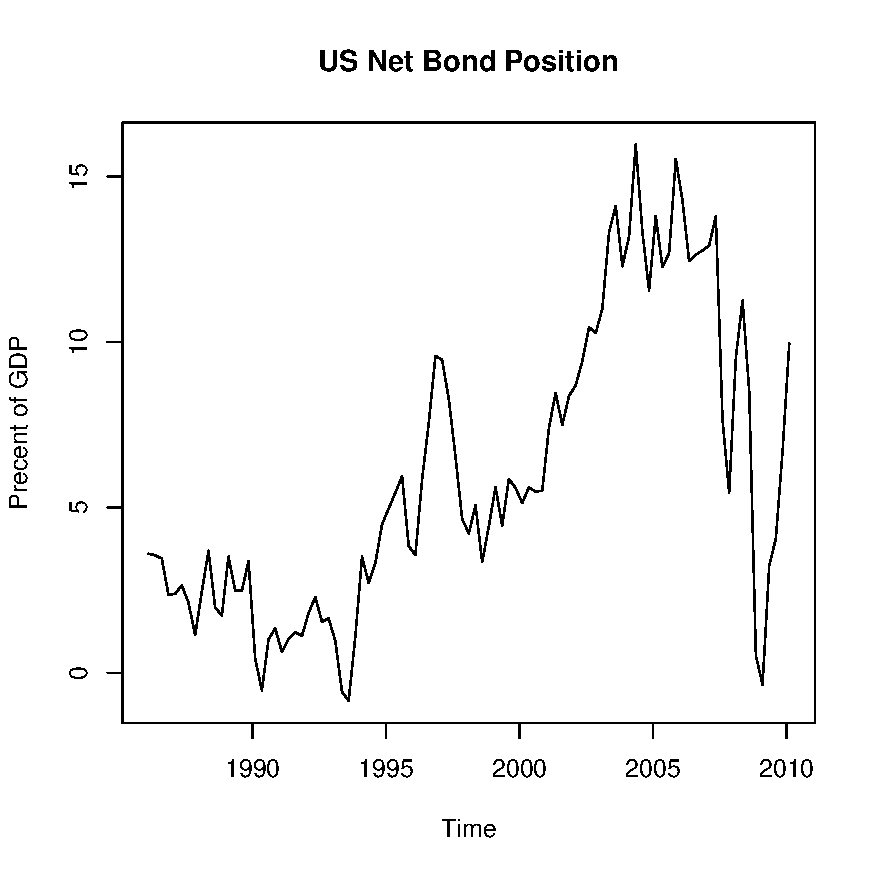
\includegraphics[scale=0.7]{bondflow}
\end{figure}

\begin{figure}[h!]
\graphicspath{{Pictures/C2/}}
\centering
\caption{Cumulative net FDI to GDP}
\label{fig:nfdi}
\includegraphics[scale=0.7] {nfdi}
\end{figure}

The evolution of foreign direct investment is also of some interest.  The cumulative net equity and net FDI series reveal the large real and portfolio flows to the US the last few years of the 1990s.  This seems to be associated with the boom in technology stocks.  The bubble burst and the NASDAQ index peaked in March 2000.   This leads to a reversal of equity and FDI flows.   The FDI data show a consistent outflow since that point which may be consistent with the offshoring that is said to have taken place in US business over the last 10 years.  Rough calculations indicate that the swing from a positive net FDI balance of 5\% of GDP in 2000 to a deficit or liability of 10\% in 2010  amounts to about \$500bn in net investment.  See Figure \ref{fig:nfdi}.

There have also been some substantial changes in speculative flows.  The SPREAD series show that the US has moved from a position of having interest rates much lower than the rest of the world at the beginning of the 1980s to being equal to slightly higher than the average of its trading partners in the more recent period.  The speculative sentiment index reveals a gradual move away from the US through the 1980s and a reversal through the 1990s but this is much more volatile and subject to short-term trends as would be anticipated.  
\subsection{Dummy variables}\label{secref:dummy}
The time series plots are also useful for identifying special situations or extreme circumstances that may not be easily understood by the model and where it may be useful to add some \emph{dummy variables}.  These are a form of \emph{transfer function} that seek to account for particular exogenous events.  It is proposed that three dummy variables be created and their ability to improve the performance of the model assessed.  The first dummy (D1) is going to cover the period from the third quarter of 1986 to the first quarter of 1988.  This is an extreme move in the variable SPREAD1 caused by a sharp movement in Mexican interest rates. This, of course, is not needed if the SPREAD2 variable that excludes Mexican interest rates is used.  The second dummy (D2) covers the period from the second quarter of 1994 to the second quarter of 1995 to cover the shock of the increase in US interest rates and the dramatic international outflows from the US bond market.   The third dummy (D3) runs from the third quarter of 2007 to the end of 2008 and represents the disturbance caused by the financial crisis. Dummies for the dot.com boom and for the 9/11 event could also be considered.  R code for dummy variables is in Appendix \ref{AppendixA} Section \ref{secref:Adummy}. 

A transfer function could also be used to account for a structural shift in the model at some point.  In this case, rather than turning the dummy on for the period of disturbance and then off again when the usual circumstances have come to an end, the transfer function is maintained.  There are no obvious breakpoints that would suggest a clear chance of a structural change.  However, it is possible to check for structural breaks at points like the introduction of the North American Free Trade Agreement (NAFTA) in 1995, the introduction of the Euro in 1999 or September 11.  This would also be one way to deal with the real risk of parameter instability. 

\subsection{Endogeneity}\label{secref:endogeneity}
The second important methodological issue is that of endogeneity.  The statistical difficulties that emerge when trying to estimate parameters when there is feedback from the dependent variable onto explanatory variables had already been noted by people like Kouri and Porter as early as 1974  \citep[pp. 464-465]{Kouri1974International} as part of their criticism of the Branson model \citep{Branson1968} and \citep{Branson1971}.  A more general explanation of issues that arise when the dependent variable is endogenous is provided by Hamilton in an analysis of the estimation of the supply and demand for oranges \citep[pp. 235-238]{Hamilton}.  

Price and quantity are determined simultaneously and are endogenous if the system is represented by two equations. 

\begin{equation}
\label{eqref:demand}
q_t^d=\beta p_t + \varepsilon_t^d
\end{equation}

For demand, with $q_t^d $ quantity demanded, $p$ price, $\beta$ the parameter to be estimated for the response of price to a change in demand and $\varepsilon_t^d$, a \emph{random variable} representing all the other factors that affect demand that have not been included. 

\begin{equation}
\label{eqref:supply}
q_t^s=\gamma p_t+\varepsilon_t^s
\end{equation} 

For supply, with $q_t^s$ the quantity supplied, $p$ is again price, $\gamma$ is to be estimated as the response of price to a change in supply, $\varepsilon_t^s$ is a random variable representing all the other factors that may affect supply but not included here.  The equality condition (supply equals demand) means that  

\begin{equation}
\label{eqref:sd}
\beta p_t + \epsilon_t^d=\gamma p_t+\varepsilon_t^s
\end{equation}

However, if Equation \ref{eqref:demand} or Equation \ref{eqref:supply} are estimated by ordinary least squares (OLS), the estimates of coefficients will be biased as the price is not independent of the error term in either case and therefore the OLS assumptions that $E[p_t\varepsilon_t^d] = 0$ and $E[p_t\varepsilon_t^s] = 0$ have been violated.    

Re-arranging equation \ref{eqref:sd} gives

\begin{equation}
\label{eqref:rdemand}
p_t = \frac{\varepsilon_t^d - \varepsilon_t^s}{\gamma-\beta}
\end{equation}

substituting equation \ref{eqref:rdemand} back into equation \ref{eqref:supply}

\begin{equation}
\label{eqref:ds}
q_t=\gamma \frac{\varepsilon_t^d - \varepsilon_t^s}{\gamma - \beta}+\varepsilon_t^s
\end{equation}

\begin{equation}
q_t=\frac{\gamma \varepsilon_t^d}{\gamma-\beta}-\frac{\gamma \varepsilon_t^s}{\gamma - \beta} + \frac{(\gamma-\beta) \varepsilon_t^s}{\gamma - \beta}
\end{equation}

and therefore

\begin{equation}
\label{eqref:ss}
q_t=\frac{\gamma}{\gamma - \beta} \varepsilon_t^d - \frac{\beta}{\gamma - \beta} \varepsilon_t^s
\end{equation}

If equation \ref{eqref:demand} is estimated by OLS, the estimate of $b_t$ would be 

\begin{equation}
\label{eqref:ols}
b_t=\frac{1/T \sum_{i=1}^{T} p_t q_t}{1/T \sum_{i=1}^{T} p_t^2}
\end{equation}

substituting equations \ref{eqref:rdemand} and \ref{eqref:ss} back into \ref{eqref:ols} gives, 

%page 234 Hamilton.  
\begin{equation}
\frac{1}{T} \sum_{i=1}^{T} p_t q_t = \frac{1}{T} \sum_{i=1}^{T} \left [ \frac{1}{\gamma - \beta} \varepsilon_t^d - \frac{1}{\gamma - \beta} \varepsilon_t^s  \right ]  \left [ \frac{\gamma}{\gamma - \beta} \varepsilon_t^d - \frac{\beta}{\gamma - \beta} \varepsilon_t^s \right ] 
\end{equation}

therefore 

\begin{equation}
\label{eqref:olsnum}
\frac{1}{T} \sum_{i=1}^{T} p_t q_t \overset{p}{\rightarrow} \frac{\gamma \sigma_d^2 +\beta \sigma_s^2}{(\gamma - \beta)^2}
\end{equation}

and 

\begin{equation} 
\frac{1}{T} \sum_{i=1}^{T} p_t^2 = \frac{1}{T} \sum_{i=1}^{T} \left [ \frac{1}{\gamma - \beta} \varepsilon_t^d - \frac{1}{\gamma - \beta} \varepsilon_t^s \right ]^2\
\end{equation}

therefore 
. 
\begin{equation}
\label{eqref:olsden}
\frac{1}{T} \sum_{i=1}^{T} p_t^2 \overset{p}{\rightarrow} \frac{\sigma_d^2 + \sigma_s^2}{(\gamma + \beta)^2} 
\end{equation}

substitute \ref{eqref:olsnum} and \ref{eqref:olsden} back into \ref{eqref:ols}

\begin{equation}
\label{eqref:sim}
b_t \overset{p}{\rightarrow} \frac{\gamma \sigma_d^2 + \beta \sigma_s^2}{\sigma_d^2 - \sigma_s^2}
\end{equation}

The estimate of $b$ is not the price elasticity of demand ($\hat{\beta}$) but an average of the price elasticity of demand $\hat{\beta}$ and the price elasticity of supply ($\hat{\gamma}$).  Therefore, if price elasticity of supply ($\hat{\gamma}$) is zero, the estimate of $b$ converges to ($\hat{\beta}$) but the larger the price effect on supply, the more biased the estimate becomes. 

Sims made an important link between the use of reduced form equations and the problems with forecasting in his seminal paper \emph{Macroeconomics and Reality} \citep{Sims1980Macroeconomics}.\footnote{The analysis was not original.  \citep{Working1925} discussed this issue when trying to determine a demand schedule for potato prices, \citep[p. 2]{Haavelmo1943} analysed the difficulty of solving simultaneous equations when there are stochastic elements, presenting Equation \ref{eqref:sim}, and \citep{Liu1960Identification}, cited by Sims, called for more complete structural models to replace the \emph{underidentified} models that had been cropped due to the statistical difficulty of assessing significance of variables when there is covariance between them. However, Sims emphasised the link between endogeneity and the poor forecasting performance of the existing models and he also proposed a solution, which is used in the work here.} 
% there is also Working (1926) and Haavelmo (1943) cited in Green.  There are also references Goldberger (1964 p. 311, Hausman (1983 pp 402-403 and Riersol (1950) in Green p 387 for VAR issues when distribution is not normal.  
This work built on the known difficulties posed by endogeneity, where there is feedback between the dependent variable and the regressors, by suggesting that there would be very few cases where true exogeneity would be present and criticising the large number of implicit assumptions that had to be made to establish supposedly \emph{reduced form} equations.  Reduced form is one that depends only on exogenous variables and past realisations of the endogenous variables.  However, in establishing these reduced-form equations decisions must be taken about which variables to include and which to exclude.  Those excluded are essentially given a zero restriction.   Sims was particularly critical of the large-scale, macroeconomic models that were built from a large number of interlocking reduced forms, arguing that the problems of endogeneity and implicit restrictions would be magnified in this case.  

To consider some of these issues in relation to exchange rate forecasting, consider the well-known and often-cited analysis of empirical tests of  exchange rate models that was undertaken by Meese and Rogoff, who found that major economic exchange rate models have no better forecasting ability than a random walk \citep{Meese1983Empirical}.  
The general equation estimated was

\begin{equation}\label{MeeseEmpirical}
s=a_{0}+a_{1}(m-m^*)+a_{2}(y-y^*)+a_{3}(r-r^*)
+a_{4}(\pi^e-\pi^{e*})+a_{5}\bar{TB}+a_{6}\bar{TB}^*+u
%there is more of this in the Froot paper%
\end{equation}

where. following Meese and Rogoff,  $s$ is the logarithm of the dollar price of the foreign currency, $m-m^*$ is the ratio of the log of the domestic to overseas money supply, $y-y^*$ is the ratio of the log of domestic to overseas income, $r-r^*$ is the short-term nominal interest rate differential, $\pi^{e}-\pi^{e*}$ is the expected long-run inflation differential and where $\bar{TB}$ and $\bar{TB}^*$ are the cumulative domestic and overseas trade balances.   Amongst the empirical work discussed, there are various methods used, including \emph{generalised least squares}, to deal with the serial correlation of the residuals and the assumption that money supply, expected long-term inflation and interest rates are endogenous \citep{Fair1970}.  There is also some allowance made for lagged adjustment. 

It is assumed that $a_{1}$ is unity in all models, the Frenkel-Bilson monetary model without sticky prices forces purchasing power parity by setting $a_{4}=a_{5}=a_{6}=0$; the Dornbusch-Frankel model allows prices to adjust gradually by setting $a_{5}=a_{6}=0$; while the Hooper-Morton model allows for the real exchange rate to adjust by leaving all the coefficients open.  These models are compared with a random walk, a random walk with drift and a VAR.  The sample is taken from March 1973 until June 1981.  Forecasts from the model are made at one, three, six and twelve month horizons.   Using mean error (ME), mean absolute error (MAE) and root mean square error (RMSE), model forecasts are compared to actual exchange rate changes and the random walk forecast.  No model achieves a lower RMSE than a random walk at any horizon.  Subsequent work by Frankel has extended the tests to monetary and portfolio balance models with limited additional success \citep{Frankel1984tests}. 
%more needed here? 

One way that Meese and Rogoff deal with the problem of endogeneity is to use instruments to try to isolate the required effect.   To return to Hamilton's orange market example, it is necessary to find a variable that will adjust with the supply curve and not the demand curve.  Hamilton suggests that in the market for oranges, the weather may be used \citep[p. 235]{Hamilton}.  As $\varepsilon_t^s$ represents all those factors that affect supply other than price, it is possible  to run the following regression. 

\begin{equation}
\label{eqref:ins}
\varepsilon_t^s = hw_t + u_t^s
\end{equation}

where h is the coefficient obtained from the regression which, by definition, is unrelated to $u_t^s$.  Going back to Equations \ref{eqref:demand} and \ref{eqref:supply}, $\varepsilon_t^d$ represents all those factors that affect demand other than price.  The weather should only affect demand via the price (as it affects supply) and therefore, should not be related to $\varepsilon_t^d$.  Changes in the price that are the result of the weather represent a shift in the supply curve not the demand curve.  

If $p^*$ is the OLS estimate of the relationship between $p_t$ and $w_t$, substitute \ref{eqref:ins} back into \ref{eqref:rdemand}, 

\begin{equation}
p = \frac{\varepsilon_t^d - hw_t -u_t^s}{\gamma - \beta}
\end{equation}

and then, as $p^*$ is the projection of $p$ on $w$.  

\begin{equation}
p^* = \frac{-h}{\gamma - \beta} w_t
\end{equation}

as $\varepsilon_t^d$ and $u_t^s$ are uncorrelated with $w_t$, 

%check u_t^s not u_t^2
\begin{equation}
\label{eqref:pp}
p=p^*+\frac{\varepsilon_t^d - u_t^s}{\gamma - \beta}
\end{equation}

Substitute \ref{eqref:pp} back into \ref{eqref:demand}, 

\begin{equation}
\label{eqref:ins1}
q_t^d=\beta \left( p^* + \frac{\varepsilon_t^d - u_t^s}{\gamma - \beta} \right) + \varepsilon_t^d
\end{equation}

and 

\begin{equation}
\label{eqref:ins2}
q_t^d=\beta p^*+v
\end{equation}

when 
\begin{equation}
v=\frac{-\beta u_t^s}{\gamma - \beta} + \frac{\gamma \varepsilon_t^d}{\gamma - \beta}
\end{equation}
%check u_t^s and not u_t^2
if $u_t^s$ and $\varepsilon_t^d$ are uncorrelated with $p^*$, $v$ is uncorrelated with $p^*$.  Now if  \ref{eqref:ins1} or \ref{eqref:ins2} are estimated  by OLS, it would provide a consistent estimate of $\beta$.

Return to \ref{eqref:ols} and use 

\begin{equation}
\hat{\beta_t^*}=\frac{1/T \sum_{i=1}^{T} p_t^* q_t}{1/T \sum_{i=1}^{T} (p_t^*)^2}
\end{equation}

\begin{equation}
\hat{\beta_t^*}=\frac{(1/T) \sum_{i=1}^T p_t^* (\beta (p_t^* + v_t)}{(1/T) \sum_{i=1}^T [p_t^*]^2}
\end{equation}
 
\begin{equation}
\hat{\beta_t^*}=\beta + \frac{(1/T) \sum_{i=1}^T p_t^*  v_t)}{(1/T) \sum_{i=1}^T [p_t^*]^2}
\end{equation}

\begin{equation}
\hat{\beta_t^*} \overset{p}{\rightarrow} \beta
\end{equation}

The process of estimating $p^*$ from the initial projection of 

\begin{equation}
p_t=\hat{\delta_I}w_t
\end{equation}

is called \emph{two-stage least squares} (2SLS) and the exogenous variable $w_t$ (weather in this case) is called the \emph{instrument} in a method of \emph{instrumental variables} where the instrument is a tool to estimate the relationship between $q_t$ and $p_t$.  The instrument must be correlated with the endogenous variable (price in this case) but not with the error term (it only affects demand through price).  

However, the big problem that is found in trying to apply this approach to the study of exchange rates is finding an equivalent of the weather for the international capital flows. The aim is to find something that will affect international capital flows but will not directly have an influence on the real exchange rate.  For example, an increased US government deficit or a changing in the credit rating could affect the net flow to the US bond market.  However, it is very likely that this would also have a direct effect on the exchange rate itself and therefore this instrument would also be related to the error term.  US corporate profitability could affect the net flow to US equities and monetary policy expectations could affect speculative flows driven by interest rate differentials, but these are sure also to affect the exchange rate. 

Finding truly exogenous variables is not easy.  Sims addressed the question of exogeneity in \emph{Money, Income and Causality} \citep{Sims1972Money}.   Sims suggested that the dependent variable be regressed on past and future values of the explanatory variables and that only if the coefficient on future values appeared to be zero could it be said that the causality was unidirectional.  If the coefficients on future values were statistically or economically significant, bidirectional causality should be assumed. This method is part of the suite of Granger-Sims causality tests that have been used to try to determine cause and effect and to test for exogeneity \citep{GrangerCause} and \citep{Sims1972Money}.    %   Need to have some of the results that have been found.  There is a section in the Palgrave book on econometrics that is useful.  

Sims used the method to assess whether money M could be called \emph{strictly exogenous} in an estimate of quarterly data of money supply and Gross National Product (GNP) for the period 1947 to 1969.    As future values of money did not appear to explain GNP he concluded that   ``The evidence agrees quite well with a null hypothesis that causality runs entirely from money to GNP, without feedback" \citet[p. 541]{Sims1972Money}.    The result was to find some support for the implicit exogeneity of the money in the \emph{St. Louis Fed reduced form equations}.\footnote{\emph{The St. Louis Fed equations} is the term given to work done using reduced-form equations by the research department at the St. Louis Fed and the broad debate about the role of fiscal and monetary policy in the business cycle.  The equations assess the relationship between government spending, money and the economy and the relative importance of fiscal and monetary action.  The original article \citep{StLouisFed} asserted that the effect of fiscal policy on the economy was relatively small and statistically insignificant.  The results were controversial and prompted a range of discussion including the argument that endogeneity of the variables meant that the estimates of the parameters established using such techniques were unreliable. Sims' contribution is a small part of this debate.} 

However, even here it may just be a matter of degree.  Clearly some aspects of monetary growth are a response to changes in economic activity and the conclusion of exogeneity may just be an artifact of the imprecision with which the test is made.  At its extreme, as \citet{Lucas1976Critique} argued, even exogenous variables can become endogenised if they become policy variables and start to affect behaviour of economic agents.  For example,  the relationship between money and economic activity can change if the monetary authorities start to change the stock of money in response to a nominal GNP target.\footnote{This is a more formal version of \emph{Goodhart's Law}, which states that statistical regularity will tend to change when a (monetary) variable is used for policy purposes  \citep{Goodhart1975Monetary}. It is part of a wider problem of feedback in the measurement and modelling of expectations which was also addressed by Sims \citep{Sims1980Macroeconomics}.}  The issue is one that is very relevant to the question of real exchange rates and capital flows because the two key instruments that the monetary authorities have to control the economy are the level of interest rates and direct intervention in the foreign exchange market.  In the former case, there will be an effect on interest rate differentials and possibly bond markets; in the latter, there will be a change in the composition of foreign exchange reserves, the central bank balance sheet and possibly also the net flow to international bond markets.   

It is hard to make the case that international capital flows are exogenous.  Any overseas transaction has to take some account of the expected change in the value of the exchange rate; the performance of the currency will also have an effect on the profitability of exporters, viability of overseas investment projects and macroeconomic variables that are important for the valuation of securities such as the effect of short-term interest rates and inflation on bonds.  In addition, the purchase of US government bonds by overseas monetary authorities is designed to ensure that a variety of other countries fix their exchange rate against the US dollar.  The factors that speculators use to assess future exchange rate movements are surely broad and ever-changing.  They must, at some point, include all the variables that have been considered for the capital-flow model.     

Granger causality tests take the form
\begin{subequations}
\begin{equation}
y_t = \alpha_0 + \sum_{i=1}^{i=p} \beta_i y_{t-i} + \sum_{j=1}^{j=p} \gamma_j x_{t-j} + \varepsilon_t
\end{equation}
\begin{equation}
x_t = \alpha_0 + \sum_{i=1}^{i=p} \beta_i x_{t-i} + \sum_{j=1}^{j=p} \gamma_j y_{t-j} + \varepsilon_t
\end{equation}
\end{subequations}

where the null hypothesis that $x$ does not Granger-cause $y$ is that the estimated value of all $\gamma$ are equal to zero.  An F-test of the null that the real exchange rate (RTWI) does not Granger-cause' the other variables is rejected.  The confirmation that changes in the value of the real exchange rate tends to lead changes in capital flows suggests a feedback from the exchange rate to capital flows that supports the use of a system-type model.   

\subsection{Vector autoregression}
This econometric technique proposed by Sims to overcome the problems caused by endogeneity and the implicit restrictions imposed on reduced form equations has come to be known as the Vector Autoregression (VAR). All the left-hand-side or dependent variables are also  explanatory variables; a wide range of variables are used; there are no initial restrictions on the parameters, including zero restrictions on the lagged variables.   The essence of the VAR is to set up a system that is made up of all the important variables, assume that they are endogenous and that there are significant lags.  Exogenous variables can be added, but these are usually restricted to things that are clearly determined outside of the system such as seasonal or special dummies, trends and constants.   The variables that will be included in the list of endogenous variables should be determined by economic theory. The lag order is eventually determined by the use of information criteria that will assess whether the addition of extra lags adds more to the explanation than it loses in terms of degrees of freedom.  

The explanation below draws on the following texts \citep[pp. 297-335]{EndersTS}, \citep[pp. 291-350]{Hamilton} and \citep[pp. 586-607]{Green}.  A simple \emph{structural} or \emph{primitive} system with just two endogenous variables and one lag would be.

\begin{subequations}
\begin{equation}\label{primitivevarone}
x_{t}=b_{10}+b_{12}y_t+\gamma_{11}y_{t-1}+\gamma_{12}x_{t-1}+\epsilon_{xt}, 
\end{equation}

\begin{equation}\label{primitivevartwo}
y_{t}=b_{20}+b_{22}x_t+\gamma_{21}x_{t-1}+\gamma_{22}y_{t-1}+\epsilon_{yt},
 \end{equation}
\end{subequations}

It is assumed that $ \epsilon_{xt}$ and $\epsilon_{yt}$ are independent of each other, are normally distributed with a constant variance.   Though the independence assumption appears quite onerous, it should be remembered that this is independence of innovation.  It does not mean that there is no relationship between the two variables ($x$ and $y$ here). A shock to either variable will have an effect on the other via the contemporaneous relationship (which is $b_{11}$ and $b_{21}$ in Equations \ref{primitivevarone} and \ref{primitivevartwo}).  As a consequence, this model cannot be easily estimated as there are feedback effects of the sort discussed above ($y_t$is related to $\epsilon_{xt}$ and $x_t$ is related to $\epsilon_{yt}$).    The variables are endogenous.  As an alternative to the use of  \emph{Instrumental Variables} the structural or primitive equations can be transformed so that ordinary least squares (OLS) can be utilised. 

In matrix form, \ref{primitivevarone} and \ref{primitivevartwo} can be written as, 

\begin{equation}
\label{transitionvar2}
\begin{bmatrix}
 1 & b_{12}\\
 b_{21} & 1
\end{bmatrix}
\begin{bmatrix}
x_{t}\\
y_{t}
\end{bmatrix}=
\begin{bmatrix}
b_{10}\\
b_{20}
\end{bmatrix}+
\begin{bmatrix}
\gamma_{11} & \gamma_{12}\\
\gamma_{21} & \gamma_{22}
\end{bmatrix}
\begin{bmatrix}
x_{t-1}\\
y_{t-1}
\end{bmatrix}+
\begin{bmatrix}
\epsilon_{xt}\\
\epsilon_{yt}
\end{bmatrix}
\end{equation}

A more general characterisation would be 

\begin{equation}\label{transitionvar}
Bx_{t}=\Gamma_{0}+\Gamma_{1}x_{t-1}+\epsilon_{t}
\end{equation}

Multiplying through by $B^{-1}$ will give the \emph{standard form of the VAR}

\begin{equation}\label{standardvar}
x_t=A_0+A_1x_{t-1}+e_t
\end{equation}

\begin{subequations}
Now with $A_0=B^{-1}\Gamma_0$, $A_1=B^{-1}\Gamma_1$ and $e_t=B^{-1}\epsilon_t$, 
and returning to the equivalent form

\begin{equation}\label{standardvarone}
y_t=a_{10}+a_{11}y_{t-1}+a_{12}x_{t-1}+e_{1t}\end{equation}

\begin{equation}\label{standardvartwo}
x_{t}=a_{20}+a_{21}x_{t-1}+a_{22}y_{t-1}+e_{1t}
\end{equation}
\end{subequations}

Now the equations can be estimated with OLS because the variables are uncorrelated with the error term.  Hamilton shows that this is the equivalent to the Maximum Likelihood Estimator (MLE) \citep[p. 293]{Hamilton}.  However, though the model can be estimated with ease, because of the transformation that has been undertaken, the coefficients that are uncovered are not those from the original structural model represented by Equations \ref{primitivevarone} and \ref{primitivevartwo}.  For the standard form of the VAR (Equations \ref{standardvarone} and \ref{standardvartwo}), the errors are a composite of $\epsilon_{yt}$ and $\epsilon_{xt}$ as $e_t=B^{-1}\epsilon_t$.  The latter can be used to uncover the components of the structural VAR from the estimation of the standard form.  However, some method must be established to deal with the problem of identification.  While it is possible to  get the estimates of $A_0$, $A_1$ and $e_t$ from Equation \ref{standardvar}, it may not be possible to get all the components of the primitive or structural model unless some restrictions are imposed.  The primitive or structural system, made up of Equations \ref{primitivevarone} and \ref{primitivevartwo}, contains eight parameters $b_{10}$, $b_{11}$, $b_{20}$,$b_{21}$,$\gamma_{10}$,$\gamma_{11}$,$\gamma_{21}$,$\gamma_{22}$ and the variance of $\epsilon_{xt}$ and $\epsilon_{yt}$, while the \ref{standardvar} VAR, made up of \ref{standardvarone} and \ref{standardvartwo}, will provide only six coefficient estimates plus the  variance and covariance of the error terms $e_{1t}$ and $e_{2t}$.  Therefore, in this case there are only nine estimates for ten parameters and a restriction will have to be made if everything is going to be uncovered.  In general, $K(K-1)/2$ restrictions will be required, where K is the number of endogenous  variables in the VAR. 

\subsection{Identification}\label{secref:ident}
There are a wide variety of restrictions that can be placed on Equations \ref{primitivevarone} and \ref{primitivevartwo}. There is a whole industry that has built up to find VAR restrictions.  These generally begin with a reference to economic theory.  For example, it is possible to assume that some of the coefficients are equal to particular values. If it were assumed that there were no contemporaneous relationship between $x$ and $y$, $b_{11}$ in Equation \ref{primitivevarone} could be set to zero; if  the contemporaneous relationship between $x$ and $y$ is assumed to be symmetrical, Equations \ref{primitivevarone} and \ref{primitivevartwo} can include $b_{11} = b_{21}$.    

One standard way to identify the VAR is to use a \emph{Cholesky decomposition} which forces the error variance-covariance matrix to become an upper triangle and therefore makes $K(K-1)/2$ restrictions as required.   This will equate the number of unknown parameters with the number of equations by imposing, virtually arbitrary, restrictions on the model.  In the example above, for Equation \ref{transitionvar2} it would be assumed that $b_{21}$ is equal to zero.  This imposes the restriction that $x_t$ does not have any contemporaneous effect on $y_t$ in Equation \ref{primitivevartwo}. Setting the restriction by using the Cholesky decomposition in this way is somewhat \emph{ad hoc} or \emph{naive} and goes some way back towards the unjustified or unsupported restrictions that were at the heart of Sims' original criticism of the endogeneity modelling problem \citep{Sims1980Macroeconomics}.  One of the main practical issues is that the results may change according to the order that the variables are placed into the VAR.  Therefore, one way to assess the resilience of the results is to shuffle the variables and to compare the findings across different specifications.  That is what is done here.  
% I am going to have to reference the sample code and the explanation when it is complete. 
 
It would be much better, if possible, to use economic theory to suggest restrictions that can be imposed on the $B$ matrix.  There is a wide literature that assesses different methods of making these restrictions.  For example, Sims proposed a six-variable VAR including variables like GNP, money supply, interest rates, inflation, investment and unemployment and made 17 restrictions that the system was \emph{over-identified}, meaning that there are more equations than unknown coefficients to be estimated \citep{Sims1986}, while Bernanke makes a number of explicit restrictions to support his assertion that the relationship between money and income is intermediated by credit rather than being the result of money illusion or causality running from income to money \citep{Bernanke1986}.  It is also possible to  place a restriction on the moving average vector of structural errors to analyse the temporary and permanent components of GNP in a two variable VAR where one additional restriction is needed for identification \citep{BlanchardQuah}.  In this way the error-convariance matrix ($\varepsilon_t$) rather than the B matrix is restricted in Equation \ref{transitionvar}. 

The Sims-Bernanke approach is adopted here.  There are are seven variables in the model being estimated. This means that  twenty one restrictions ($K(K-1)/2$) are needed for system identification.    
It is now possible to consider the economic arguments for restrictions and to impose these on the model.  For example, in this paper, there will be seven variables which can be represented by seven equations along the lines of Equations \ref{primitivevarone} and \ref{primitivevartwo} where there is a seven-by-seven B matrix like that in Equation \ref{transitionvar} and Table \ref{tabref:svar1} is the first matrix of Equation \ref{transitionvar2}.  Table \ref{tabref:svar1} gives an overview of of the restrictions suggested.  

 
\begin{table}[t]
\begin{threeparttable}
\caption{SVAR Restrictions}
\begin{tabular}{p{4cm} rrrrrrrrr}	
  \hline
 &  CNB & CNE & CNFDI & COT & RTWI & SPREAD & S1 \\ 
  \hline
  CNB & 1 & NA & 0a & 0b & 0c & NA & 0d\\ 
  CNE & NA & 1 & NA & 0e & NA & 0f & NA\\ 
  CNFDI & 0g & NA & 1 & 0h & NA & 0i & 0j\\ 
  COT & NA & 0k & 0l & 1 & NA & 0m & NA \\ 
   RTWI & 0n & NA & NA & NA & 1 & NA & NA\\ 
  SPREAD & NA & 0p & 0q & 0r & NA & 1 & 0s\\ 
  S1 & 0t & NA & 0u & NA & NA & 0v & 1\\ 
   \hline
\end{tabular}
\label{tabref:svar1}
\begin{tablenotes}
\small
\item The table shows the individual equations in the VAR and the restrictions that are placed on some of the coefficients to identify the system.  Reading across the page, the first row reads CNB as the dependent variable, NA for CNE meaning that this coefficient can be estimated, there is a zero restriction placed on CNFDI and the letter identifies the explanation for the restriction in the paragraph below.  
\end{tablenotes}
\end{threeparttable}  
\end{table}

\subsection{VAR restrictions}\label{secref:varres}
The following are the explanations for the twenty-one restrictions that are imposed on the VAR.  Note that these are contemporaneous restrictions (same quarter), a lagged effect is still allowed.  The equations are read across rows, with the dependent variable normalised to unity, coefficients on independent variables that are to be estimated are labelled "NA" in Table \ref{tabref:svar1}, as they are in the R code, and the zero restrictions are labeled alphabetically.  The matrix does not have to be symmetric; for example, a change in cumulative net foreign direct investment to GDP (CNFDI) may affect speculative sentiment in the current quarter, as the confidence expressed by international investors may encourage speculative activity, but that does not mean that an increase in speculative sentiment has to affect CNFDI which may be expected to be influenced by factors that are more long-term or fundamental in their nature.   R code for the restricted matrix is presented in Appendix \ref{AppendixA} Section \ref{secref:AppSVAR}. It will be evident that the B matrix is set up like Table \ref{tabref:svar1}.   

Reading across the row for each equation in turn. The cumulative net bond equation (CNB) is restricted by imposing a coefficient of zero on the influence of foreign direct investment (a), cumulative official treasuries (b), real exchange rate (c) and sentiment (d).  Though the exchange rate and speculative sentiment could increase net bond flows, it seems more likely that this would happen at the short end of the yield curve (and therefore would be better captured by the money market proxies SPREAD or S1 ) and, as noted in \citep[p. 3]{Siourounis2004Capital} and \citep{HauEquity}, most of the international bond flows appear to be hedged against foreign exchange gains and losses.    The cumulative net equity equation is restricted only at the cumulative official treasuries (e) and the interest rate spread (f).  Lower relative rates could inspire a more positive attitude towards corporate profits, but rate changes could just as likely be a response to broad-based economic weakness that would not be conducive to profitability. The restrictions on the FDI equations are on bond flows (g), official treasuries (h), the interest rate spread (i) and sentiment (j).  As foreign direct investment is assumed to be a more long-term commitment, it seems likely that short-term relationship with other variables will be modest; the longer term coefficients can play a more prominent role.   The flow of Official Treasuries (COT) is most likely to be a response to an appreciation of the US dollar and therefore should not be significantly affected by things like equity (k) and FDI (l) flows, unless indirectly.  The real exchange rate is allowed to be affected by all the other variables outside of net bond flows (n).  The interest-rate spread, which presumably is largely a function of central bank policy, is restricted against net equity (p), net FDI (q), official purchase (r) and sentiment (s).  The exchange rate and net bond flows are allowed to have some influence.  Finally, the sentiment equation is restricted on bonds (t), FDI (u) and the spread (v), but is allowed to be affected by equity and the exchange rate.  This allowed for some positive spillover from more optimistic attitudes towards the economy, which may affect the flow of money to the stock market or into real investments.   It also allows for positive feedback from a change in the value of the exchange rate to speculative sentiment. 

It is, of course, possible to argue about some of the restrictions that have been imposed here.  However, at least the restrictions are out in the open, can be debated and can be assessed against the available data evidence.  This marks an improvement on the \emph{ad hoc} or \emph{naive} methods.  It is  of course possible to run the model, assess the outcome and then make adjustments to the restrictions.  However, this would increase the risk of \emph{data mining} or \emph{over-fitting} and it is not done here.  However, as a robustness check, three models are assessed:  the first is one that is restricted using the Cholesky decomposition (called System One); the second takes a random ordering of the variables and again restricts the coefficients on the lower triangle to be zero (called System Two); the final version uses the structural restrictions noted above (System Three).  If all three methods give similar results, there should be greater confidence that the outcome is not just a function of the ordering of the variables or the assumptions that have been made. % reference code.  

% I think that this must go later as a justification for the model. 
%\begin{table}[ht]
%\begin{threeparttable}
%\caption{SVAR Estimation}
%\begin{tabular}{lrrrrrrrrr}	
% \hline
% & CNB & CNE & CNFDI & COT& RTWI & SPREAD1 & S1 \\ 
 %\hline
 % CNB & 1.00 & -0.01 & 0.00 & 0.00 & 0.00 & 0.20 & 0.00 \\ 
 % CNE & 0.08 & 1.00 & 0.20 & 0.00&  -0.03 & 0.00 & 0.02 \\ 
 % CNFDI & -0.00 & 0.11 & 1.00 & 0.00 & -0.03 & 0.00 & 0.00 \\ 
 % COT & -0.02 & 0.00 & 0.00 & 1.00 & 0.09 & 0.00& 0.20\\
 % RTWI & 0.00 & 0.21 & 0.09& 0.31 & 1.00 & 0.07 & 0.27\\ 
 % SPREAD1 & -0.02 & 0.00 & 0.00 & 0.00 & 0.04 & 1.00 & 0.00\\ 
 % S1 & 0.00 & 0.07 & 0.00 & 0.17 & 0.01 & 0.00 & 1.00 \\ 
  % \hline
%\label{tabref:svar2}
%\end{tabular}
%\begin{tablenotes}
%\small
%\item The table shows the estimated coefficients for the A matrix which allows contemporaneous relationships between the variables to be identified.   
%\end{tablenotes}
%\end{threeparttable}  
%\end{table}

%Table \ref{tabref:svar2} reveals the estimated coefficients for the estimation of the equivalent of equations \ref{SVARone}, \ref{SVARtwo} and \ref{SVARthree}.  It is possible to read across the rows to understand the contemporaneous relationship between variables (including the restrictions that have been placed on the model.  For example, most of our interest is on the real exchange rate.  It is possible to read across the fifth row and see that the model does a relatively successful job of explaining the contemporaneous relationship between the real exchange rate and capital flows\footnote{the signs must be reversed from those in the table because the equation is currently of the form $Ax_t=\Gamma_0 +\Gamma_1x_t-1+e_t$ as in equation \ref{transitionvar2} and \ref{transitionvar}.}.   The negative relationship between the exchange rate and the interest rate spread is consistent with uncovered interest parity.  Given that sentiment is based on the purchase of other currencies, the evidence is consistent with the expected short term relationship between speculative flows and the real exchange rate.   There is a negative relationship between the flow in the holdings of official treasuries and the real exchange rate. This is likely to be a consequence of a overseas central banks being prompted into intervention in the foreign exchange market by the weaker US dollar.  The negative relationship between the real exchange rate and the net inflow to equities and bonds is not what would have been expected.  The estimated effect of the bond flow is small and consistent with evidence that many international bond portfolios hedge their bond exposure.  The equity flow warrants additional investigation.  

\section{Results}\label{secref:varresults}
The main results for System Three are presented in Figure \ref{fig:IRF1} where it is evident that the most dramatic and significant contribution to the change in the real exchange rate comes from the two types of speculation that are analysed.  \emph{Impulse Response Functions}, to be discussed more fully in Section \ref{secref:IRF} below, show that a one unit innovation or shock to the S1 series, equal to a ten percentage point change in the net position of speculators relative to the total speculative position, will have on average a positive effect of close to 4\% on the real trade-weighted exchange rate over the next eight quarters.  The 95\% confidence intervals, denoted by the red, dashed lines, reveal that it is very likely that there is a positive effect.  For speculative flows that are linked to the interest rate differential, a one-unit or one hundred basis-point improvement in US interest rate advantage tends on average to have an effect of increasing the US real trade-weighted index by about 10\%.  Here there is more uncertainty and there are times when the effect is quite minimal. 

For the other major flows, there is a great deal more ambiguity.  The effect of a one-unit increase in the net cumulative bond position relative to GDP (equivalent to about \$35bn at the beginning of 2010) is close to zero over the following four quarters and slightly negative beyond that point.  The impulse response functions show a range of possible outcomes that are centred around zero.  The average effect of an innovation to the net inflow to US equities of one percentage point of GDP or about \$35bn is on average zero but the confidence intervals are wide, suggesting that sometimes the equity inflow is associated with an appreciation of the real exchange rate and sometimes with a depreciation.    The net flow associated with foreign direct investment is very similar, but slightly more positive,  to that of equities.  The action of overseas central banks, cumulative official treasuries (COT),  is associated with a positive effect of an average 4\% over the next four quarters.    Here the causation is likely to be running from the exchange rate to inflows as the overseas central banks respond to US dollar weakness by buying dollars and US government bonds to help to maintain their exchange rate pegs.  The width of the confidence intervals indicates that there are many occasions when the capital flow associated with central bank intervention does not have the desired effect and weakness in the US real trade-weighted index continues.   

The overall impression is one where speculation has a much more precise and significant effect on the real exchange rate than the other capital flows.  It is clear that speculation can have a effect that is not just short-term in nature and that this can have a real effect on the economy.  A very similar pattern is noted in the impulse response functions that are derived from the other Systems (see Figures \ref{fig:IRF2} and \ref{fig:IRF3} and Section \ref{secref:IRF2} below).  The results are robust to alternative specifications.  This increases the confidence in the results as it appears that it is not the method of identifying the VAR or the restrictions that have been imposed having a major effect on the outcome.  

The rest of this section provides more detail of the analysis behind the results briefly presented here including the model selection, diagnostic tests and the creation of impulse response functions.  The statistical analysis is carried out in the R environment \citep{R}. \footnote{See http://www.R-project.org/ for more details. The packages xtables, dse and vars were primarily used for compiling tables in La Tex and for running the VAR analysis \citep{R}, \citep{xtable}, \citep{varsa} and \citep{varsb}}  
% does this whole section go earlier? More is needed on R.  Does it come generally earlier with an overview of the vars package here? 

\begin{landscape}
\begin{figure}[t]
\graphicspath{{Pictures/C2/}}
\centering
\caption{Impulse Response Functions for RTWI for System Three}
\label{fig:IRF1}
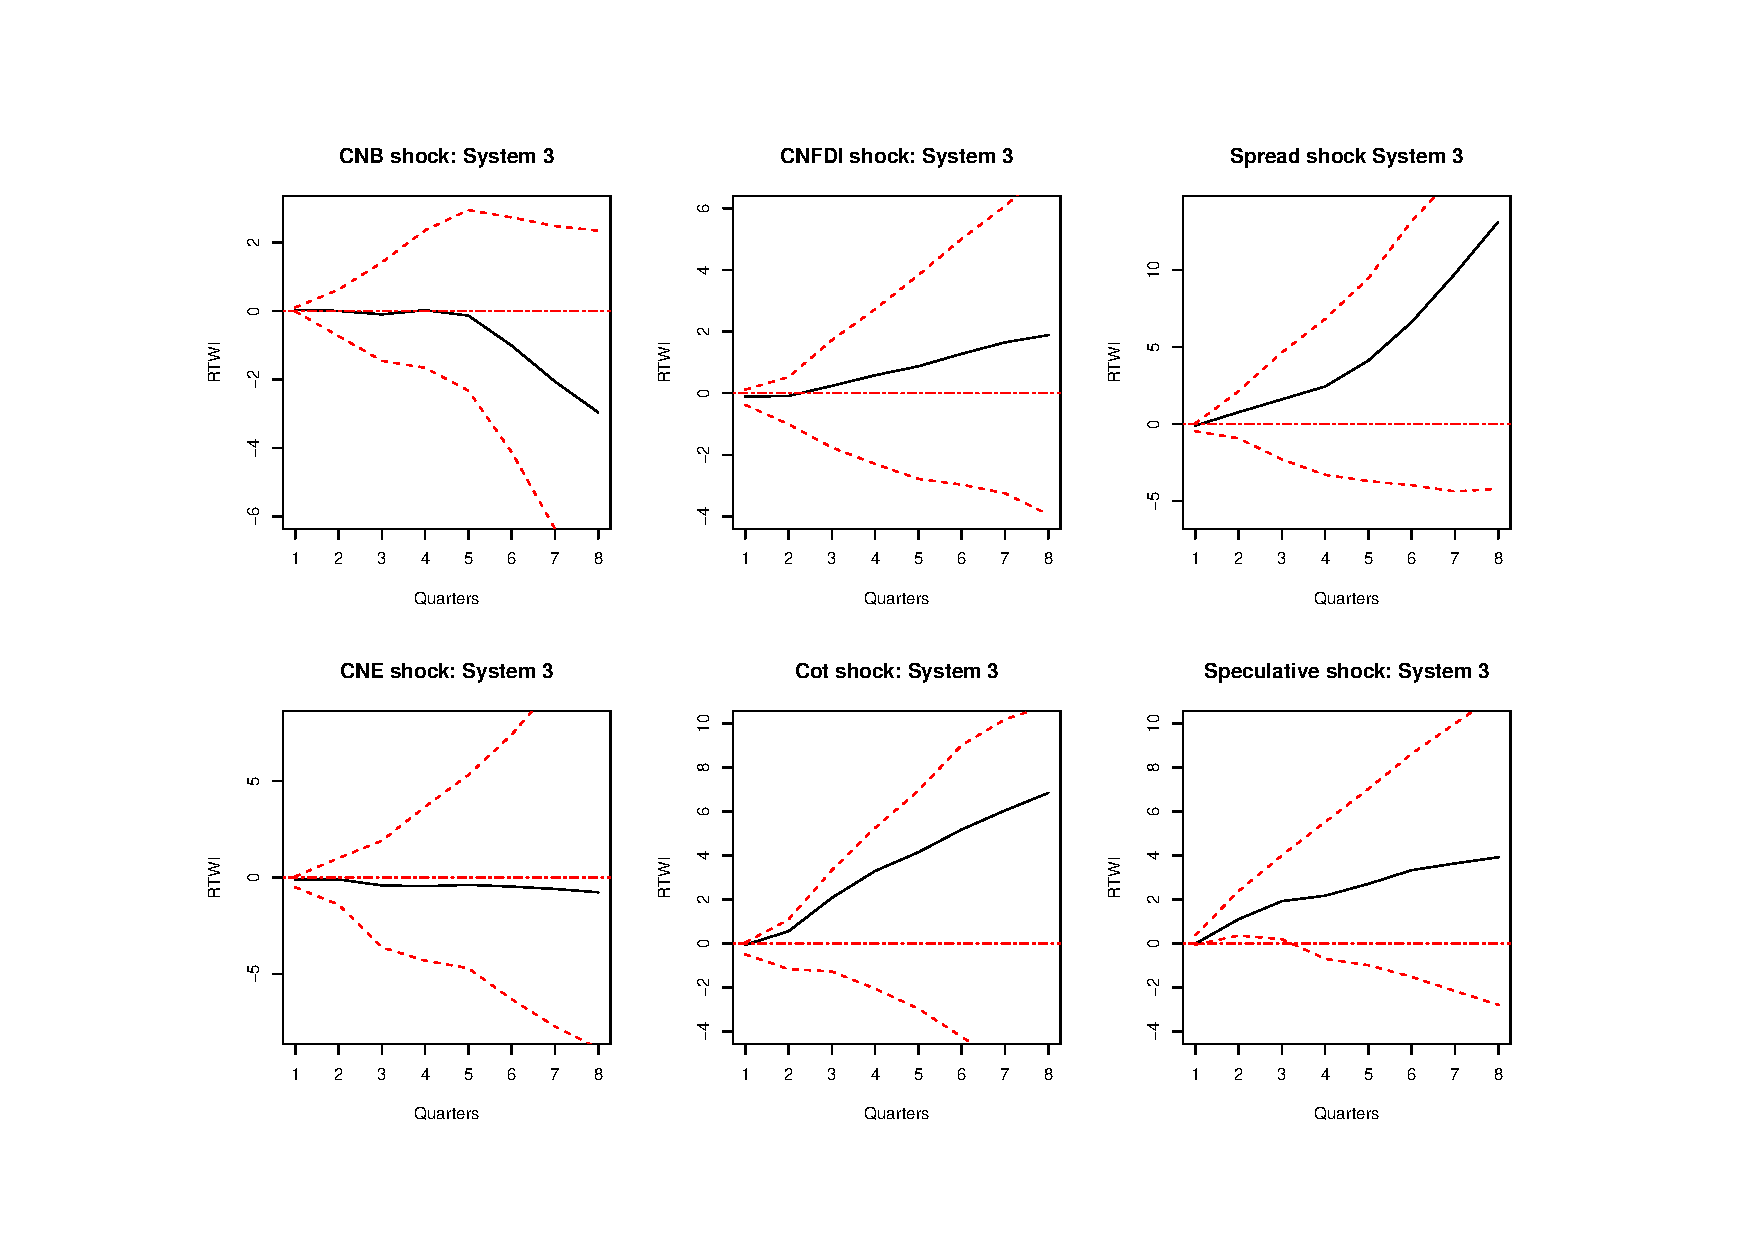
\includegraphics[scale=0.8]{IRF3}
\end{figure}
\end{landscape} 



\subsection{Model selection}\label{secref:modelsel}
The are a number of different models to be assessed.  There are various ways that the exchange rate  (nominal or real), interest-rate spread (SPREAD1 or SPREAD2) and sentiment (S1 or S2) can be measured.  There are also the three proposed solutions to the non-stationary current account series and also the possibility of the addition of exogenous variables to the VAR.  The three dummy variables have already been set up for specific period of volatility in international capital flows can be included if they add explanatory power.   The issue of a structural break has also been considered and there is also some room for seasonal dummies.  In addition, the VAR can include a constant or a trend.  

Table \ref{tabref:model} presents the key information for the baseline model selection process.  The three main models are identified by the inclusion of the net cumulative current account (CCA), the change in the net cumulative current account (DCCA) or the absence of th net cumulative current account ("No Current Account").  Models are tested with and without dummy variables.  The log likelihood and the Akaike (AIK) and Bayesian information criteria (BIC) are reported along with a number of diagnostic tests.  See Appendix \ref{AppendixA} Section \ref{secref:Adiag} for full details of the R code use to select variables from the raw data files and for carrying out the diagnostic tests. 

Table \ref{tabref:model} shows a comparison of the different models that are proposed.  
Information criteria are used for model selection and for choosing the length of the lags to include.  The Likelihood function is the probability that the parameters of the model are observed given values of the variables in the system and a probability density function.  Parameters can be adjusted to maximise the likelihood.  In which case, it is usually easier to use the log of the likelihood function.  However, the more parameters are added to the model, the higher the Likelihood function as each new series is sure to add something.  Therefore, in order to guard against over-fitting, it is usual to place a penalty on the use of additional explanatory variables. 



% re-think this table.  It show the diagnostic statistics but would it be better just to compare the models and they consider the diagnostics for the one that is tested?  Add in the new models with S2 and Spread 2 and combinations.  
\begin{landscape}
\begin{table}
\begin{threeparttable}
\caption{Model Selection}
\begin{tabular}{p{5cm}rrrrrrrrr}
  \hline
 & Model 1 & Model 2 & Model 3 & Model 4 & Model 5 & Model 6 & Model 7 & Model 8 \\ 
  \hline
  CCA                          & Yes    & Yes         & No     & No    & No           & No    &  No     & No  \\ 
  DCCA                       & No     &  No         & Yes    & Yes   & No          & No     & No      & No  \\ 
  No CA                      & No     &  No        & No      & No   & Yes         & Yes    & Yes     & Yes \\  
  Dummy                     & No     &  Yes       & No     & Yes   & No          & No     & Yes     & Yes \\
  Lag Length               &   4      &  4         & 4         & 4      & 1            &  4       & 1        & 4\\ 
  Lag Length: AIC                     &    3     &  3          & 3         & 3      & 1            & 1        & 1       &  3 \\ 
  Lag Length: BIC                     &   1      &  1          & 1         & 1      & 1             & 1       & 1        & 1\\ 
  Log Likelihood                  & -1693.94  & -1627.99 & -2365.93& -2305.49 & -1598.27 & -1413.18  & -1555.74 & -1358.10  \\ 
  AIC                           & 19.4501   & 18.6721 & 33.7877 & 33.0450  &  14.7446   & 14.7887  & 14.2961 &  14.1583\\
  BIC                           &  21.6783 & 21.6529  & 36.1546  &  36.108  &  16.4275   & 16.5043 & 16.5399 & 16.4895\\
 Roots                        &  Good       &  Good      & Good       & Good     & Good         & Good    & Good        & Good \\
 Serial Correlation.                     &    564.23   & 575.54     & 567.54  & 589.07  &  314.02      & 389.15  &  338.09    &394.06  \\
   (p-value)                            &  (0.00)      &  (0.00)    & (0.00)   &  (0.00)  &  (0.00)       & (0.00)     & (0.00)      & (0.00) \\
 Hetroskedasticity.                          	 &  3060         &  3060       & 3060     & 3060     & 2576       &    2492         & 2576       & 2492     \\
  (p-value)                         & (0.00)         & (0.00)       & (0.00) & (0.00)    & (0.00)      & (0.00) & (0.00) & (0.00) \\
Normality              		&990.0	   &  36.81   &  1438.00  &  18.49       &  2401      &  1469   &  210.00       &   32.43   \\
  (p-value)                            &    (0.00)    &   (0.00)   &   (0.30)   &  (0.00)   &  (0.00)   &  (0.00)   &   (0.00)  & (0.00) \\
 \hline
\label{tabref:model}
\end{tabular}
\begin{tablenotes}
\small
\item The models are versions of Equations \ref{standardvarone} and \ref{standardvartwo} estimated with OLS.  CCA, DCCA and No Current Account identifies the three main class of model (with the net cumulative current account, the change in the net cumulative current account and without the current account variable).  Dummy indicates whether the dummy variables are included.  Lag length is the lag length used and the following rows indicate the lag length indicated by the Information criteria (Akaike Information Criterion (AIC) \citep{AIC} or Shwartz Bayesian Information Criterion (BIC) \citep{BIC}.  Log Likelihood is the log likelihood of the VAR estimation.   ``Roots'' checks for stability with the result of a test that the roots of the coefficients of the autoregressive polynominal lie outside the unit circle.   Serial correlation, hetroskedasticity and Normality are the residual tests of the null hypothesis that normal, independent and identically distributed.   Serial correlation is tested using the multivariate Portmanteau and Breusche-Godfrey test; hetroskedasticity is tested using the ARCH-LM test; the test of normally distributed errors is the multivariate Jarques-Bera test of the null that all the residuals are normally distributed. 
\end{tablenotes}
\end{threeparttable}  
\end{table}
\end{landscape}

 There are  a number of ways that the Likelihood function can be adjusted to penalised taking additional variables into account.  The two used in this study are the Akiake Information Criterion (AIC) \citep{AIC} and the Bayesian Information Criterion (BIC) \citep{BIC}.  The AIC is 

\begin{equation}
AIC=2k-2ln(L)
\end{equation}

where k is the number of parameters in the model and L is the maximised value of the likelihood function.  The BIC is 

\begin{equation}
BIC= kln(n) - 2ln(L)
\end{equation}

with n being the number of observations in the model.

The AIC tends to apply a small penalty to additional parameters while the BIC is less generous.  As a result it is often the case that the two methods can suggest different solutions.  The AIC is likely to favour a model with more explanatory variables and the BIC is likely to suggest something more parsimonious.  This is the case in Table \ref{tabref:model} where AIC indicates that that Model 8 with dummy variables and four lags (but no current account) is the best fit while the BIC suggests that Model 5 is the best, with no current account, no dummies and only one lag. 

\subsection{Model specification and diagnostics}\label{secref:ass} 
%Add here the note in \citep[p.47]{Juselius2007Cointegrated} that simulaton studies have shown that the statistical inference is much more susceptible to parameter instability, autocorrelation and residual skew than it is to hetroscedasticity and kurtosis.   
The preferred model, according to the range of information and diagnostics outlined in Table \ref{tabref:model} is the one that does not include the current account, has four lags and uses the three dummy variables, SPREAD2 and S1.  A model with a linear trend and a constant is the one that produces the lowest values of the AIC and BIC.  The summary information on model 8 reveals that the system is stable as the roots of the autoregressive coefficients are all within the unit circle.  The dummy variables are significant. 
  
There is some concern that the diagnostic tests for the preferred model indicate that there is serial correlation of the residuals, hetroskadasticisty and that the errors are not normally distributed.  \citep[p.47]{Juselius2007Cointegrated} reports simulation studies that have shown that the statistical inference for VARS is much more susceptible to parameter instability, autocorrelation and residual skew than it is to hetroskedasticity and kurtosis.   Each of these can be considered in more detail in turn.

There are two tests of serial correlation.  The first is the \emph{Lagrange Multiplier} test that is sometimes called the \emph{Breusch-Godfrey} test after its authors \citep{Breusch1979} and \citep{Godfrey1978}. The test is based on an initial estimation of the autocorrelation of the residuals. 

\begin{equation}
u_t = A_0 y_{t-1} + A_1 y_{t-2}...+ B_0 u_{t-1} + B_1 u_{t-2}...+ \varepsilon_t
\end{equation}
Once the lag length is determined, the null is a test of whether all the B values are equal to zero.  Formally, the test is
\begin{equation}
LM_h = T(K - tr(\Sigma_R^{-1} \Sigma_e))
\end{equation}  

where  $\Sigma_R$ and $\Sigma_e$ are the covariance matrices of the restricted and unrestricted models respectively.  Asymptotically, the test statistic has a $\chi^2$ distribution with degrees of freedom equal to the lag length multiplied by the square of the number of endogenous variables.  \citep{EG} present a small-sample adjustment that is used here. See \citep[p. 29]{varsb} for full details.  The results of the test are presented on line 12 of Table \ref{tabref:model}.  This shows that in each case the null hypothesis that all the residuals are different from zero is rejected.  This is a little surprising as the \emph{correlograms} of the estimated residuals from each of the equations do not show any serial correlation in any of the equations (see Figure \ref{fig:acf}.  These are constructed as the \emph{autocorrelations} of the residuals of each of the estimated equations.  The autocorrelations are constructed as the ratio of the covariance between the current residuals and each lag normalised to the estimated variance of the residuals.  Therefore the covariance is,

\begin{equation}
\sum_{i=1}^{i=j}\hat{(e_t)(e_{t-i})} = T^{-1}\sum_{t=1}^{t=T}(e_t -\overline{e})(e_{t-i} - \overline{e})
\end{equation}    

where $j$ the order of covariance to be estimated, and the variance is 

\begin{equation}
\hat{\sigma_e^2} = T^{-1}\sum_{t=1}^{t=T}(e_t -\overline{e})^2
\end{equation}
See \citep[pp. 13 - 14]{HarveyTSM} for more details.  

According to the assumptions that were used to construct the VAR, these covariances should be zero, though this will not be the case in the sample.   To test the null hypothesis that the assumption is correct, confidence intervals are drawn according to the formula $\frac{z_{1-\alpha/2}}{\sqrt{N}}$ where $z$ is the quantile function from the standard normal distribution, $\alpha$ is the confidence level (usually set at 5\%) and $N$ is the number of observations.  This is an approximation and assumes a normal distribution.  The limits for a 5\% confidence at drawn in Figure \ref{fig:acf} in blue.   

\begin{figure}[h!]
\graphicspath{{Pictures/C2/}}
\centering
\caption{Autocorrelation of residuals}
\label{fig:acf}
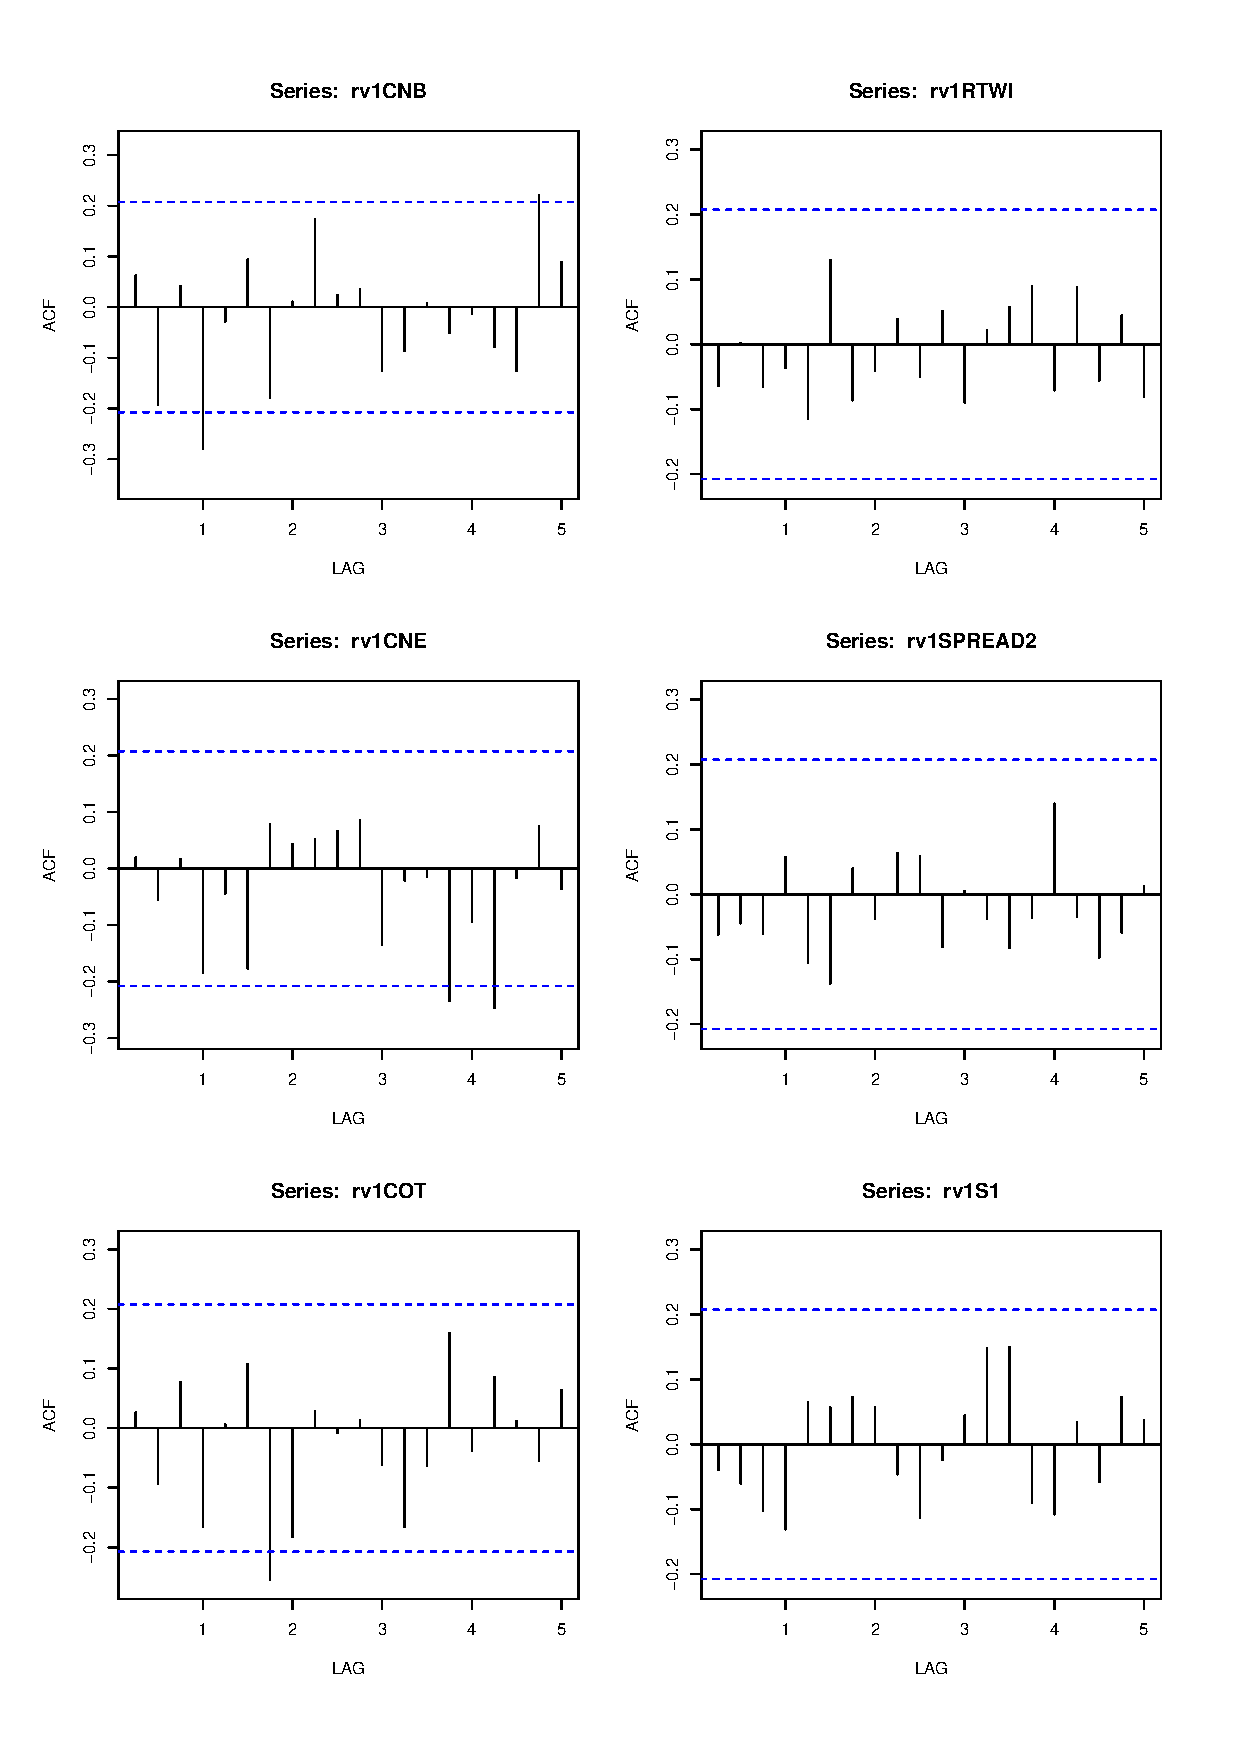
\includegraphics[scale=0.6] {acf}
\end{figure}

The test of hetroskedasticity is based on the following regression. 
\begin{equation}\label{eqref:het}
vech(\hat{u_t}\hat{u_t}') = \beta_0 + \beta_1 vech(\hat{u}_{t-1}\hat{u}_{t-1}')...\beta_q vech(\hat{u}_{t-q}\hat{u}_{t-q}') + v_t
\end{equation} 

Where $vech$ is the half-vectorisation of the symmetric matrix $(\hat{u}_t\hat{u}_t')$.\footnote{Half-vectrorisation is the stacked lower triangle.  For example, $\begin{pmatrix} a & b \\ c & d \end{pmatrix}$ would be $\begin{pmatrix} a \\ c \\ d \end{pmatrix}$.}  The null hypothesis of no hetroskedasticity takes the form $H0:= \beta_0 = \beta_1 = \beta_2 =...=\beta_q = 0$ with the test statistic. 
\begin{equation}
VARCH_{LM}(q) = \frac{1}{2} T K(K +1)R_m^2
\end{equation}
where 
\begin{equation}
R_m^2 = \frac{2}{K(K+1)}tr(\hat{\Omega}\hat{\Omega}^{-1})
\end{equation}
With $\Omega$ the variance-covariance matrix from Equation \ref{eqref:het}.  The test is distributed as $\chi^2 (qK^2(K + 1)^2/4$.  See \citep{Hamilton} for more details.   The test statistic is recorded in line 14
of Table \ref{tabref:model}.  This shows some evidence of hetroscedasticity in the preferred model.  However, the univariate tests indicate that this comes from the SPREAD2 equation.  The null of uniform variance cannot be rejected for any other series. This is also evident from the time series plot of the residuals (see Figure \ref{fig:tsresid}).

Hetroskedasticity could be addressed by some sort of adjustment such a taking logs or using the Box-Cox transformation \citep{BoxCox}.  However, with many of the capital flows negative, it would be necessary to transform the data first by adding sufficient to take them into positive territory.  This would change the relationship between different capital flows and would affect the reading of the results. \footnote{The transformation should involve adding sufficient to the raw data to take them into positive territory.  Logs can then be taken and the data analysis carried out on the transformed figures.  Once results are achieved, the data can be transformed back to original values for the interpretation.}   
 
\begin{figure}[t]
\graphicspath{{Pictures/C2/}}
\centering
\caption{Time Series of Model Residuals}
\label{fig:tsresid}
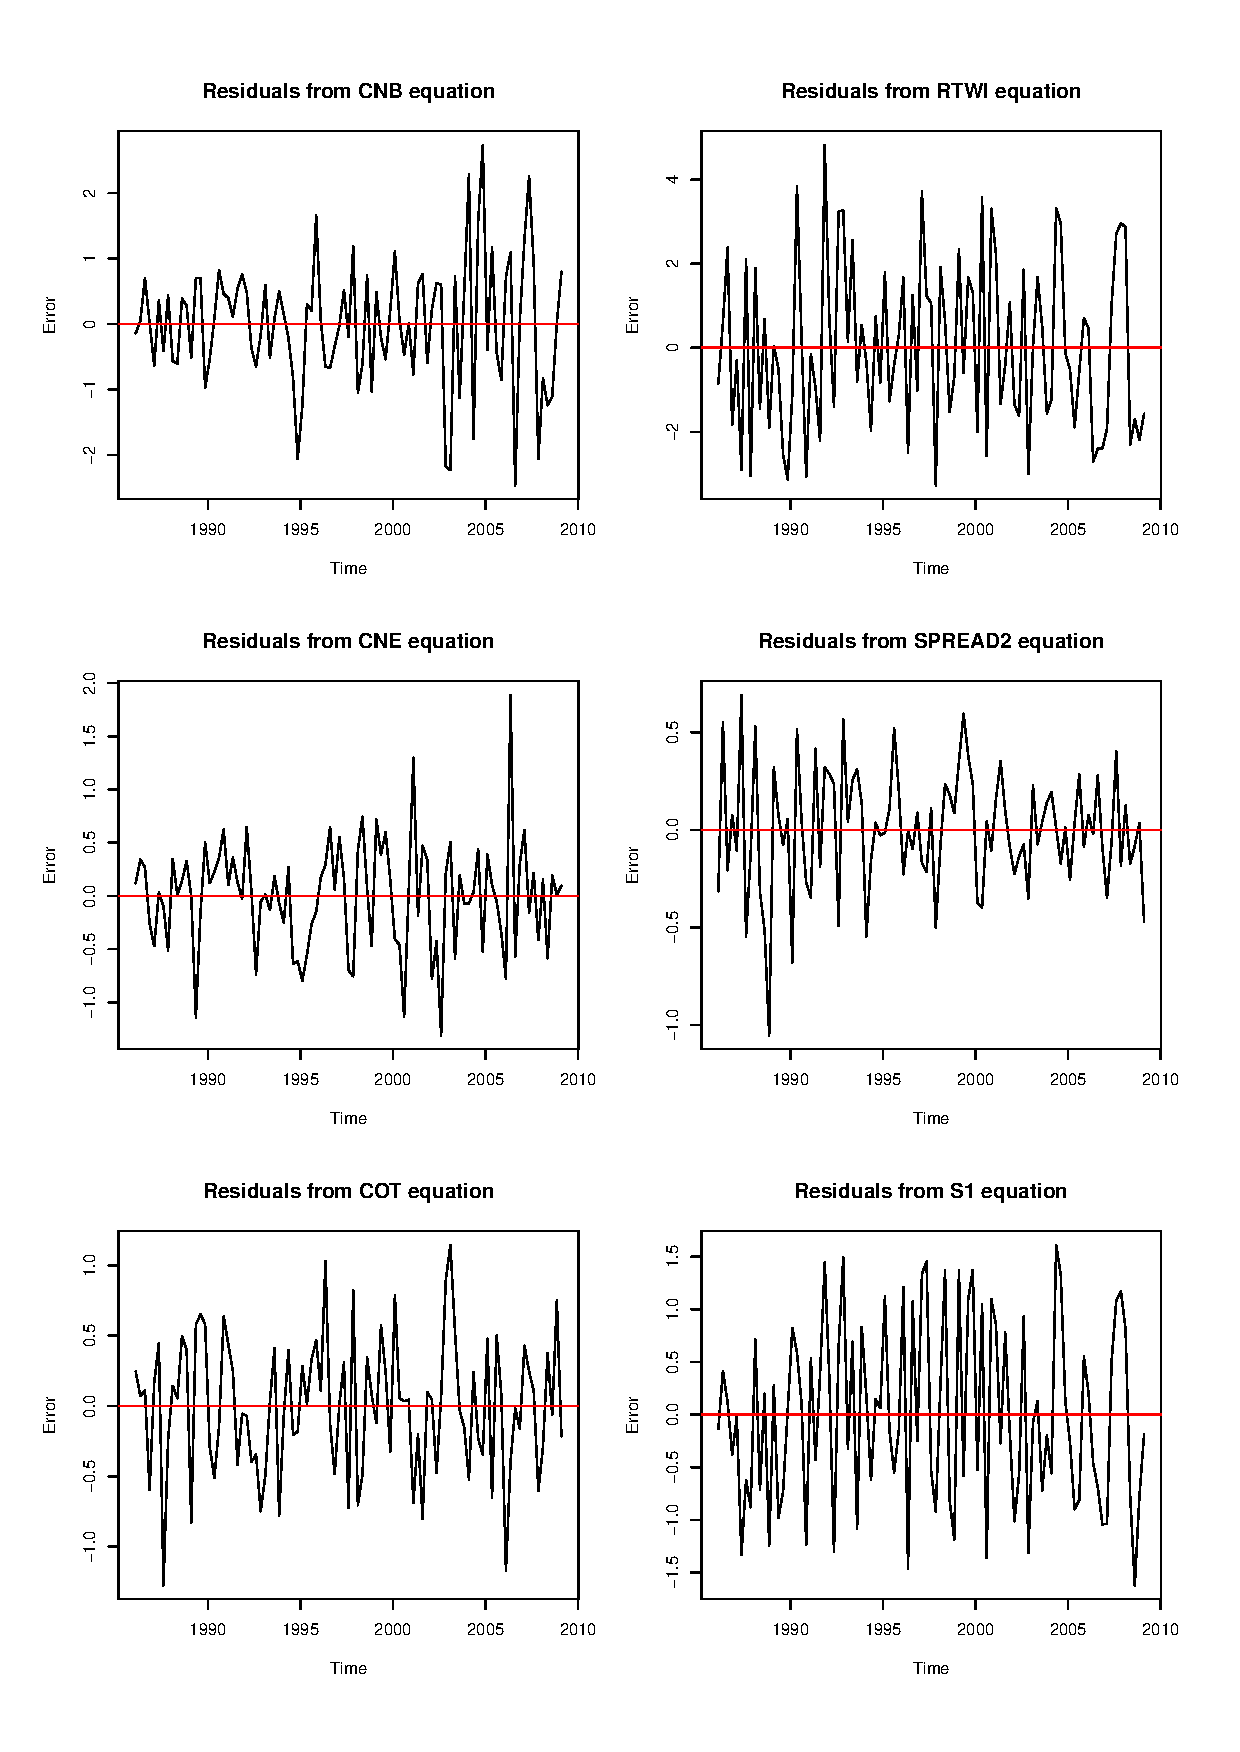
\includegraphics[scale=0.6] {residts}
\end{figure} 

The Jarque-Bera Test is used to test whether the residuals from the regression are normally distributed \citep{JB1980}, \citep{JB1981} and \citep{JB1987}.  The test takes the form. 
\begin{equation}
JB_{mv} = s_3^2 + s_4^2
\end{equation}
where $s_3$ is the \emph{sample skew}, defined as 
\begin{equation}
s_3^2 = Tb_1b'_1/6
\end{equation}
and $s_4^2$ is the sample kurtosis,
\begin{equation}
s_4^2 = T(b_2 - 3K)'(b_2 - 3K)/24
\end{equation}
where $b_1$ and $b_2$ are the third and fourth non-central moment vectors and K is the number of endogenous variables \citep[p. 31]{varsb}.  The tests are presented separately in row denoted normality of Table \ref{tabref:model}.  It can be seen that the null hypothesis that the distribution is free from skew is not rejected but the null of normal kurtosis is rejected.  The univariate tests reject the null of normality for the CNE and CNFDI series.   This is also evident in Figure \ref{fig:histresid}.

\begin{figure}[ht]
\graphicspath{{Pictures/C2/}}
\centering
\caption{Histogram of model residuals}
\label{fig:histresid}
\includegraphics[scale=0.6]{hresid}
\end{figure}   
%Something about the overall weakness of the system is needed at some point.  The method relies on parameters of the model being stable through the whole of the period under study.  This is not likely to be the case when there have been such tremendous changes in the international capital environement. 

\subsection{Parameter stability}
One of the problems with use of the VAR methodology is the assumption that the parameters are stable over time.  Given the tremendous changes that have taken place in the international financial markets, this assumption is not likely to hold.  It is evident from Figure \ref{fig:tsresid} that there has been a large increase in the size of the international capital flows that are associated with net international bond flows.  The increase in official purchase reflects the increase in activity from central banks trying to fix their exchange rates.  One way to deal with this would be to use a model that incorporates time varying parameters.  There are examples of these \emph{state space} or \emph{Bayesian Vector Auto Regression} models, but these are not followed here. 

An \emph{Empirical fluctuation process} is used to test for model stability.  The \emph{generalised fluctuation test} uses an empirical model to construct boundaries that mark the limit of what can be considered stable.  The test is on the null hypothesis that the estimated coefficients of the VAR are stable over time.  $H0:= \beta_1 = \beta_2 = \beta_3 \ldots+\beta_T = \beta$.  As common, the residuals are investigated for departures from the assumptions of the model.  Investigating the cumulative sum of the ordinary least square residuals (OLS-CUSUM) is more sensitive to small changes or gradual changes in the underlying parameters of the model \citep{BrownCUSUM}.  The residuals can be standardised or squared for different forms of the test.    The recursive residuals are calculated as  

\begin{equation} 
\hat{u_i} = \frac{y_i - x'_i \hat{\beta}^{(i-1)}}{\sqrt{1 + x'_i (X^{(i-1)} X^{(i-1)})^{-1} x_i}} \: \: \: \:  (i = k+1,...,n),
\end{equation}

where each estimate $\hat{u_i}$ is on the series up to point $i$, $X^{(i-1)} = (x_1, x_2...x_{i-1})$.  Under the null hypothesis the $\hat{u_i}$ fluctuate around zero with an independent distribution of $N(0, \sigma^2)$.  
 
These should fluctuate around zero.  If there is a structural break, there will be a deviation from zero that breaks the defined boundary at the point of the break.  The OLS-CUSUM empirical fluctuation process is defined by 

\begin{equation}
W_n^0(t) = \frac{1}{\hat{\sigma}\sqrt{n}}\sum_{i = 1}^{nt} \hat{u_i} \: \: \: \: (0 \leq t \leq 1),
\end{equation}

The test for stability is based on a departure from zero that is as probable as the power of the test to be applied $(\alpha)$.  If the evolution of the squared residuals is assumed to be a normal Gaussian process,  $E[W_n^0(t)] = 0, V(W_n^0(t) ) = i-k$.    The standard deviation of the process is $\sqrt{i - k}$.  It is usual to define the boundary above and below zero half way between k and T with probability equal to $\alpha$ to define the rejection of the null that the model is structurally stable.  In this case, $\alpha$ is set at 0.05 and is identified by the red, dashed lines in Figure \ref{figref:cusum}.  See \citep{strucchange} for more details on the test and its implementation. 

\begin{figure}[h!]
\graphicspath{{Pictures/C2/}}
\centering
\caption{Cumulative sum of residuals stability test}
\label{figref:cusum}
\includegraphics[scale=0.5] {stab}
\end{figure} 


 \subsection{Impulse response functions}\label{secref:IRF}
Once the base VAR model has been decided, it can be used to assess how variables in the system interact.  This is most usually done by creating \emph{Impulse Response Functions} (IRF).  These are the graphical representations of the effect of a one unit shock or innovation on one part of the system to any other part of the system.  The IRF show how the system deals with disturbances.  Technically, this is achieved by using the moving average (MA) version of the VAR and then applying some restrictions to ensure that the shocks can be identified.  

The \emph{Wold moving average representation} is used to turn a stable\footnote{Stability requires that roots of the AR process, $I - A$ in this case, lie outside the unit circle such that the AR element is less than unity.  This has been checked by noting that the roots of the characteristic polynomial are outside the unit circle, see \citep[p19-20]{HarveyTSM} for more details.  All the unit roots for all the equations have been checked. See line "Roots" in Table \ref{tabref:model}.} AR process into one that is MA.   See \citep[p. 17]{HarveyTSM}, \citep[pp. 64 - 70]{Hamilton} or \citep[pp. 307-311]{EndersTS} for full details. 
   
Starting from the standard VAR representation of Equation \ref{standardvar}, 

\begin{equation}
x_t=A_0+A_1x_{t-1}+e_t
\end{equation}

by iterating backwards, this becomes  

\begin{equation}
x_t=A_0 +A_1(A_0 + A_1 x_{t-2} + e_{t-1}) + e_t
\end{equation}

so 

\begin{equation}
x_t=(I+A_1)A_0 + A_1^2 x_{t-2} + A_1 e_{t-1} +e_t
\end{equation}

after n iterations

\begin{equation}
x_t=(I+A_1 + \ldots + A_1^n)A_0 + \sum_{i=1}^n A_1^i + A_1^{n+1} e_{t-n-1}
\end{equation}
% check this last equation
and therefore, given that $A_1$ is less than one as a result of the stability assumption, shocks will have a diminished impact over time as $A_1^n$ will tend to zero as n tends to infinity.  Meanwhile, $(I+A_1 + ... + A_1^n)A_0$ is the mean value of the endogenous components.  Therefore, 

\begin{equation}
x_t=\mu + \sum_{i=0}^{\infty} A_i^i e_{t-i}
\end{equation}

Where $\mu$ is the mean level of $y$ and $z$ in the original Equations \ref{primitivevarone} and \ref{primitivevartwo}. 

Once the estimates of $A_1$ have been made, they can be used to assess the effect of a shock or innovation from one series in the VAR on any of the others.    However, as discussed in Section \ref{secref:ident} the system is underidentified and therefore some restrictions have to be imposed if the original, structural relationships are to be assessed.  In this case, the identification requires that $A_1$ be replaced by the $B^{-1}A_1$.  Which would be 

\begin{equation}
x_t=\mu + \sum_{i=0}^{\infty} \Phi_i \varepsilon_{t-i}
\end{equation}

when

\begin{equation}
\Phi_i=\frac{A_1^i}{1 - b_{12}b_{21}}
\begin{bmatrix} 1 & -b_{12} \\ -b_{21} & 1 
\end{bmatrix} 
\end{equation}

because the IRFs are now based on the structural errors rather than those of the standard form.  Now it is evident that a one-unit shock to $\mathbf{\varepsilon_t}$ will increase $\mathbf{x_t}$ by $\sum_{i=0}^{i=n}\Phi_i$ where $n$ is the number of periods to look forward.  

However, if the system is underidentified (as discussed in Section \ref{secref:ident}) this will not be possible because not all the components of $\Phi_i$ will be available.  This is where it becomes necessary to make some restrictions to ensure that the system is identified. 

Therefore, if $b_{21}$ is set to zero (ideally because it is deemed plausible due to economic theory), there will be no contemporaneous relationship between a shock to $y_t$ and $z_t$.  However, there will still be lagged effects as $y_{t-1}$ will affect $z_t$.  The impulse response function will trace out the effect of a shock to one variable on another variable in the system.  Because the system is assumed to be stable these shocks will gradually diminish over time.  For example, if the auto-regressive coefficient is 0.8\%, meaning that the initial shock on a univariate series would increase the dependent variable $y_t$ by one unit contemporaneously, 0.8\% in the period after the shock and by 0.64\% two periods after the shock.  

The path of the shock can be displayed in a diagram to show the average effect that is expected given the estimated parameters.  However, it must be noted that the parameters are estimated with some imprecision and therefore it is usual to also draw some confidence intervals around the path to show the range of possible outcomes that the system suggests is most likely.  Therefore, the IRFs show the most likely effect that a shock to one variable will have on one of the other variables and also the range of possible outcomes.   

\subsection{Confidence intervals}
There are two methods for constructing the confidence intervals.  The first is to assume that the error in estimating the coefficients of the system is normally distributed and to use this together with the estimate of the standard error to draw 95\% confidence intervals in the usual way.  However, with multicollinearity within the system and some evidence that some of the error terms are not normally distributed (see Section \ref{secref:ass}), it is better to use the underlying data to assess the precision of the IRFs by using the \emph{bootstrap method}.  

The boostrap first presented by Efron \citep{Efron} is a modification or simplification of the \emph{jacknife} method which samples from the sample.  While the jacknife systematically excludes one element of the sample, bootstrap takes a random sample from the sample with replacement.  In this way the sample is taken as the population and repeated estimates are made of the parameters of interest allowing empirical estimates of the qualities of the estimation to be made.  

In this case, the \emph{residual bootstrap} is used.  This involves using a random draw of the residuals from the estimated system, calculating estimated values of the endogenous variables and then re-estimating the coefficients of the system before calculating the IRF.   If this is done 100 times, the empirical distribution can be used to identify the central 95\% (or any other level of precision that is required) of the estimates and use this to define the confidence intervals.  

In a simple univariate system, 

\begin{equation}
y_t = b_0 y_{t-1} + e_t
\end{equation} 

can be estimated to get values of  $\hat{b_0}$ and $\hat{e_t}$.  These are then used to construct $\hat{y_t}$ from the estimates ($\hat{y_t} = \hat{b_0}y_{t-1} + \hat{e_j}$) where $\hat{e_j}$ is drawn randomly (with replacement) from the sample of $\hat{e_t}$.   These estimates of $y_t$ are used to make a new estimate of the system parameters and these are used to calculate new IRF.  The process is repeated a large number of times.  

The one complication with the multivariate system is the likelihood that shocks to the system may not be independent and in this case it would be better to randomly draw sets of shocks or innovations or to daw one innovation and use that to calculate the contemporaneous errors.  There were one thousand bootstraps in this study.  The confidence interval was set at 95\% so that once the IRF are ranked the $50^{th}$ marks the 5\% confidence interval and the $950^{th}$ marks the 5\% confidence interval.\footnote{in the R package VARS \citep{varsa} and \citep{varsb} the function IRF is used to create impulse response functions from the standard or structural VAR.  Options for the function allow estimation of bootstrap or standard confidence intervals. If bootstrap is selected, the number of draws can be specified.  The larger the number of samples, the more precise the estimate but the greater the computational cost.  See Appendix \ref{AppendixA} Section \ref{secref:AIRF} for R code that will calculate the IRF from each of the estimated VAR models.}  See Figure \ref{fig:IRF1}, \ref{fig:IRF2} and \ref{fig:IRF3} for IRF and confidence intervals for the three systems that have been estimated.  

\subsection{Alternative models}\label{secref:IRF2}
As has  been discussed in Section \ref{secref:ident}, there are some questions about the use of the naive method of  identifying the standard VAR model so that the structural IRF can be estimated.  In particular, the ordering of the endogenous variables becomes important and this feels unsatisfactory.  The Structural VAR method that imposes theory-related restrictions is more satisfying but there remains a risk that the system will be mis-specified if the restrictions turn out to be incorrect.  

As a result, it was decided that there would be three different systems used to identify the VAR:  System One will force the B matrix to be a lower triangle based on the initial order of the endogenous variables (the order is that of Table \ref{tabref:svar1}); System Two is the same but the order of the variables is selected randomly (see Appendix \ref{AppendixA} Section \ref{secref:systemtwo} for more details of the method, the R code and outcome of this random selection); System Three is the Structural VAR (SVAR) and the restrictions fully discussed in Section \ref{secref:varres}.  If the three different systems produce three different results then it can be concluded that the method used for identification plays a large part in the results.  This would raise doubts about the reliability or robustness of the results. However, the results are very similar.  The IRF for the three systems are presented in Figures \ref{fig:IRF1}, \ref{fig:IRF2} and \ref{fig:IRF3} respectively.  

The aim of this study is to get some understanding of the forces that can drive the real exchange rate from its equilibrium level. Therefore, the main focus here is the effect of an innovation from capital flows to the real exchange rate, and therefore these are the main IRFs that have been drawn.  The IRF show the effect of a one-unit shock or innovation for one component of the system to all the other parts of the system (see Section \ref{secref:IRF} for a full discussion of the construction of IRFs and the confidence intervals).  Remember, when considering the economic significance of these shocks, that in the standard model, capital flows are measured as percentage of nominal GDP which is \$3.6 trillion in the first quarter of 2010.  Therefore, a shock or innovation to bonds (CNB), equity (CNE) or FDI (CNFDI) is the equivalent of about \$35bn at present.  A one-unit change in the exchange rate index represents an adjustment of about 1\% given the index fluctuates more-or-less around 100.  An innovation for the Spread series means a 1-percent or 100 basis point increase in US short-term interest rates relative to those in the rest of the world.  An innovation for the speculative-sentiment index means that there has been a ten-percentage point increase in speculators holding US dollars with a short position in either Euro, GBP, CHF or JPY.  

It is possible to look at the relationship between some of the other components of the system.  For example, IRF of the effect of a one-unit shock to the flow associated with speculative sentiment has a near 1\% positive effect on the net inflow to the US bond market and for FDI but has very little effect on net equities.  A shock to sentiment has close to \% cumulative effect on the interest rate spread.  This, together with the information about the relationship between speculative sentiment and FDI, suggests that this speculative sentiment reflects some broad attitude towards the US economy and economic conditions.  As would be expected, when there is a shock to speculative momentum there is an outflow of official funds from the US bond market:  overseas central banks do not need to support their currencies by buying US dollars and bonds when there is positive speculative sentiment to support the US dollar.  It is reassuring that these IRFs are coherent and consistent with economic theory.  

\subsubsection{System three:  structural VAR}
As discussed in Section \ref{secref:varresults}, Figure \ref{fig:IRF1} shows the impulse response of a one unit shock from each of the variables in the VAR on the RTWI using System Three for the identification.  The most significant findings are that a one-percentage-point increase in the relative interest rate spread has a cumulative effect of over 10\% on the RTWI over the two years following this shock and that this effect is most likely to be between -5\% and 12\%.  This is a series that is designed to capture short-term money market flows, including those associated with the carry trade\footnote{The carry trade is discussed more fully in Chapter \ref{Chapter4} but basic ideas is that there is borrowing in a relatively low interest rate currency and investment in a relatively high interest rate currency with the aim of making more on the interest rate differential than is lost in the exchange rate adjustment.} attempt to take advantage of the breakdown in UIP.  It is notable that the effect of the interest-rate spread is large and significant even when other flows that may be affected by interest rates, such as bond or equity, are taken into account.  The effects are consistent with evidence from Chapter \ref{Chapter4} that UIP does not hold.  The evidence is also consistent with the Dornbusch over-shooting model that was discussed in Section \ref{secref:money}.  This model suggests that there will be an immediate jump in the exchange rate in favour of the currency with the increase in relative interest rates so that there can be a subsequent reversal to provide a capital loss to offset the income gains from the interest-rate differential \citep{Dornbusch1976Expectations}.  However, it is evident from the IRFs that the adjustment is not instantaneous and there is scope to achieve some initial capital gains as the investment currency appreciates to augment the income gains from the relatively high interest rate.  The pattern is consistent with the idea that increased interest rates can encourage carry trade activity that will have a positive near-term effect on the exchange rate that would undermine UIP in the short-run but may increase the risk of sharp reversals further out.  The carry trade will be discussed more fully in Chapter \ref{Chapter4}.   

The speculative sentiment series may also capture some of the carry trade effect as well as momentum and other speculative activity.  Figure \ref{fig:IRF1} shows that, using the identifications of System Three, a ten percentage point increase in speculative sentiment (S1), meaning the net position of speculators relative to total speculative positions, has an average 4\% effect on the real exchange rate over the next 2 years.  In the short-run (out to three quarters) the effect is positive in about 90\% of the cases.   This is the strongest results (in terms of statistical significance) from all the IRFs reported here.  The result indicates that speculative activity can have real effects, even outside the very short-run. Given the effect of the real exchange rate on other parts of the economy, it indicates that speculative activity can have real effects on economic activity. 

The influence of the other types of capital flow on the real exchange rate are less clear cut.   This may not be surprising given the method employed and the nature of these capital flows.  The VAR tries to find parameters for the relationships between the series that are stable for the whole of the period under study.  Though the analysis of the stability of the system that was conducted was reasonably encouraging (see Figure \ref{figref:cusum} for the graph of the cumulative sum of the residuals) given the tremendous changes that have taken place in international financial markets between 1986 and 2010, it is very likely that relationships have changed over time.   This is part of the reason that the confidence intervals are so wide.  One way to deal with this would be to allow the coefficients to change over time by estimating a model with  time-varying parameters (TVP).  For an example of a Bayesian Vector Auto Regression (BVAR) that uses state-space methods for TVP see \citep{DelNegroFRBNY}.  There are fuller details in \citep{KoopMethods}.  This is an extension that will be made in future research.    	
%more..

When using System Three for identification, the influence of net bond flows on the real exchange rate is minimal.  The effect of a one unit innovation on net international bond flows (CNB) could be between -2\% and +2\% but is on average close to zero.  The result is the same as that found in \citep{Siourounis2004Capital}.  The finding are consistent with the belief that international bond portfolios tend to hedge their activity.  This means that for a capital inflow that comes from the bond market, there is an offsetting outflow in the form of a forward rate agreement or swap that will set the price at which the foreign currency receipts will be translated back into domestic currency. In this case, there should be no net effect. \citep[p 3]{Siourounis2004Capital} cites a survey in \citep{HauEquity} of proprietary data from a \emph{fund of funds} that reports international bond flows to over 100 funds are hedged in more than 90\% of the cases compared to just 12\% in equities.    

For the identification of System Three, a shock to the net international flow of equity (CNE) has virtually no effect on average over the 2 years.  However, the confidence intervals are wide (between plus and minus 7\%) indicating a variety of effects at different times.    The result is something of a contrast to the much more positive relationship established between equity flow and the exchange rate that was found in \citep{HauEquity} and  \citep{Siourounis2004Capital}.  These each found a large and significant effect on the exchange rate from equity flows.  The limitations of the VAR method outlined above may be at work here.  The other studies used nominal rather than real rates and did not include any variables to represent speculation.  As such, it may be the case that other studies are picking up some of the effects of speculation when they find that net equity flows have a significant effect on the exchange rate.  

An innovation in the net flow of foreign direct investment (CNFDI) has a small, positive but imprecise effect on the real exchange rate.  Intuitively, the effect of net foreign direct investment is likely to be more ambiguous given the uncertainty about what it means for exchange rate flows.  There are two main ways that international transactions of this category can be completed:  paying cash and paying with equity.  In the first case there could be a foreign exchange transaction if the acquiring company does not have existing resources or ability to borrow in target currency; in the latter case there is no foreign exchange change unless the receivers of the script sell it to change foreign currency proceeds back into domestic currency.  There are also leads and lags and timing issues that suggest a lot of imprecision in the estimation of the effect of this type of flow on the real exchange rate.   

An unexpected increase in net official purchase of US bonds (COT) has a positive effect on the US real exchange rate.  This indicates that overseas central banks are able to reduce the  upward pressure on their currencies through their intervention in the foreign exchange market (buying US bonds in the process).  

 
\begin{landscape}
\begin{figure}[t]
\graphicspath{{Pictures/C2/}}
\centering
\caption{Impulse Response Functions for RTWI for System One}
\label{fig:IRF2}  
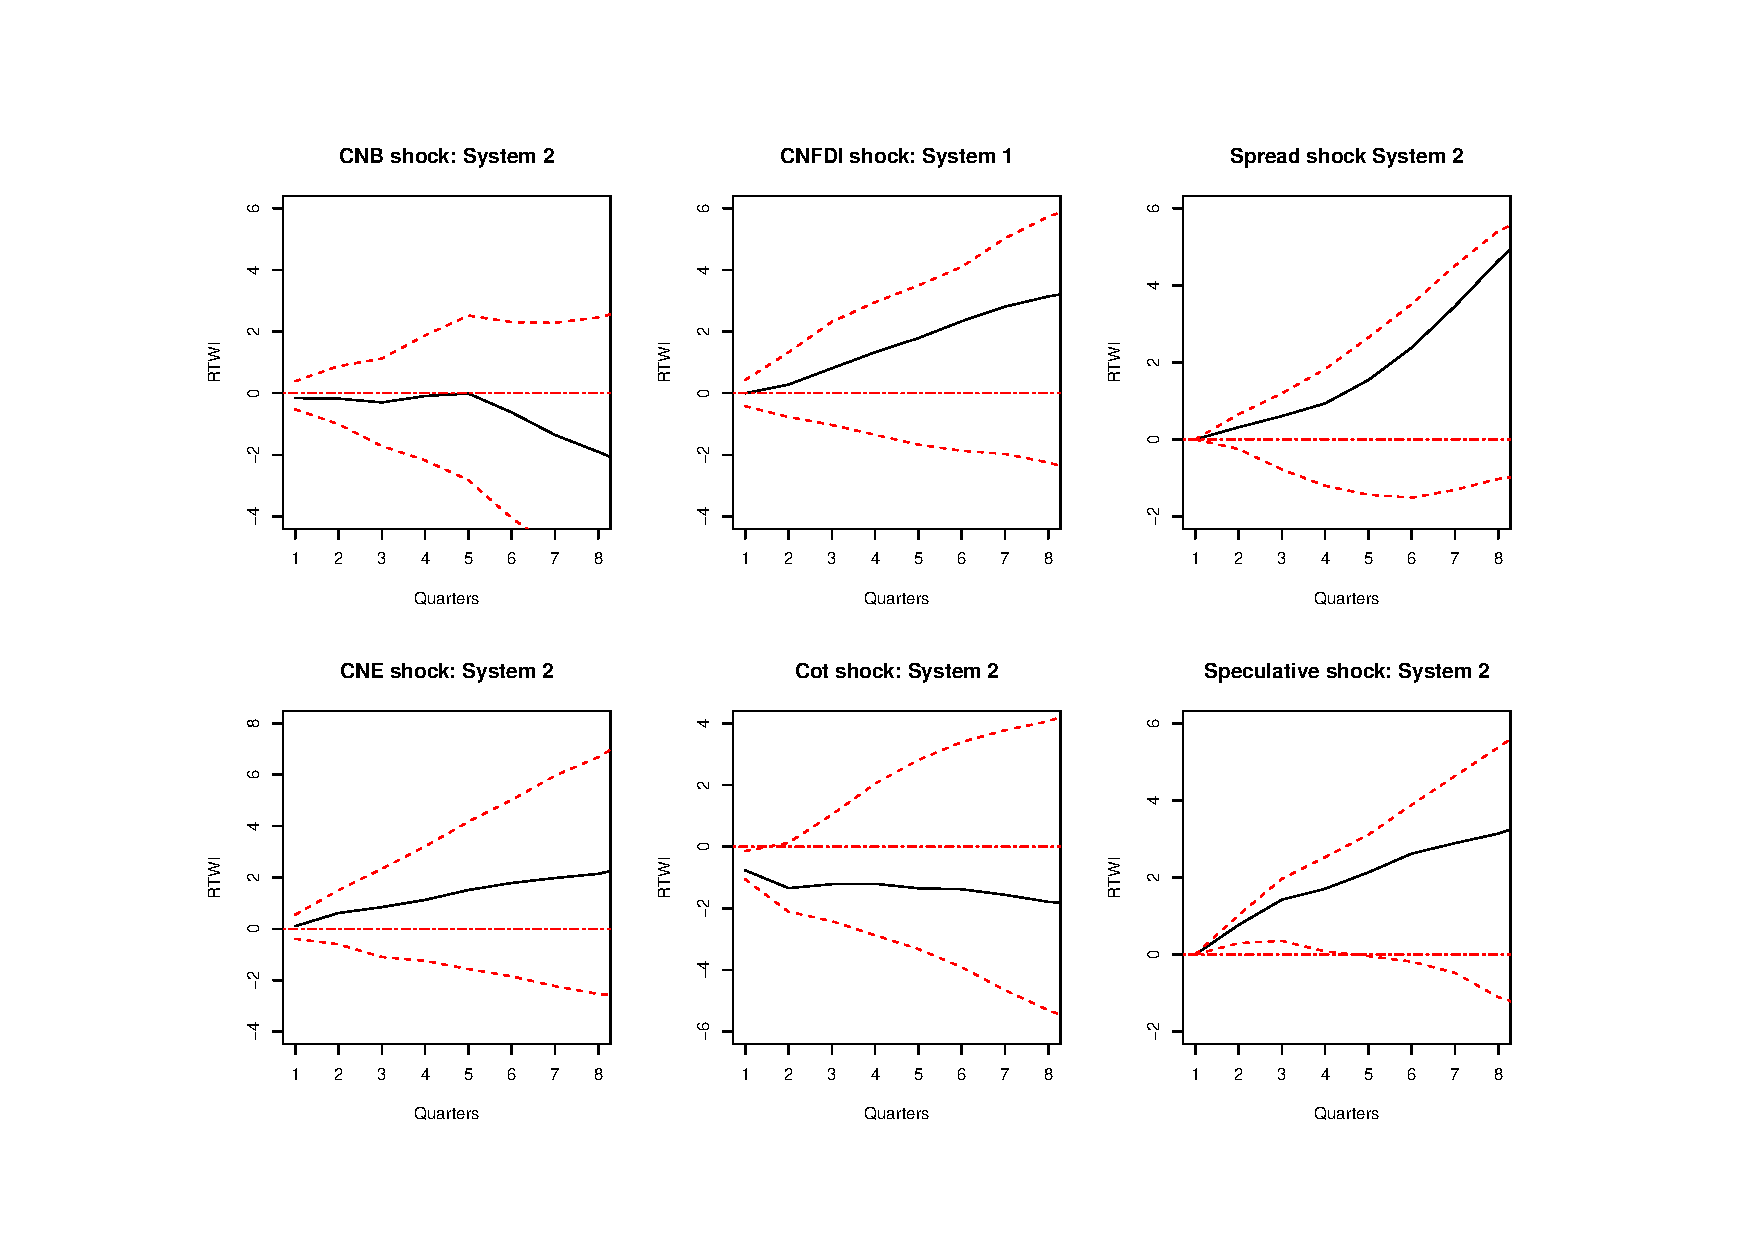
\includegraphics[scale=0.8]{IRF1}
\end{figure}
\end{landscape}

\subsection{Comparison of identification methods}
It is encouraging that the broad patterns identified in the IRFs remain very similar no matter which of the three methods is used to identify the system (see Figures \ref{fig:IRF1}, \ref{fig:IRF2} and \ref{fig:IRF3} for IRFs created with Systems 1, 2 and 3 respectively).  The speculative effects related to sentiment and interest rate differentials are unequivocally positive in all three cases. The other major effect that is identified is that of the positive relationship between the official purchase of treasuries and the exchange rate.  The different methods of identifying the system all indicate that the other capital flows have a very uncertain effect on the real exchange rate.  

The one difference that is evident in the IRF from the three different system is that for System One the initial impact of a positive shock to the purchase of bonds by foreign official institutions is negative and then turns positive in line with the other two systems.  This may be the result of reverse causation as it is most likely that the foreign exchange intervention will take place at times of US dollar weakness as, by definition, this is the time when overseas currencies are appreciating against the US unit. 

\begin{landscape}
\begin{figure}[t]
\graphicspath{{Pictures/C2/}}
\centering
\caption{Impulse Response Functions for RTWI for System Two}
\label{fig:IRF3}
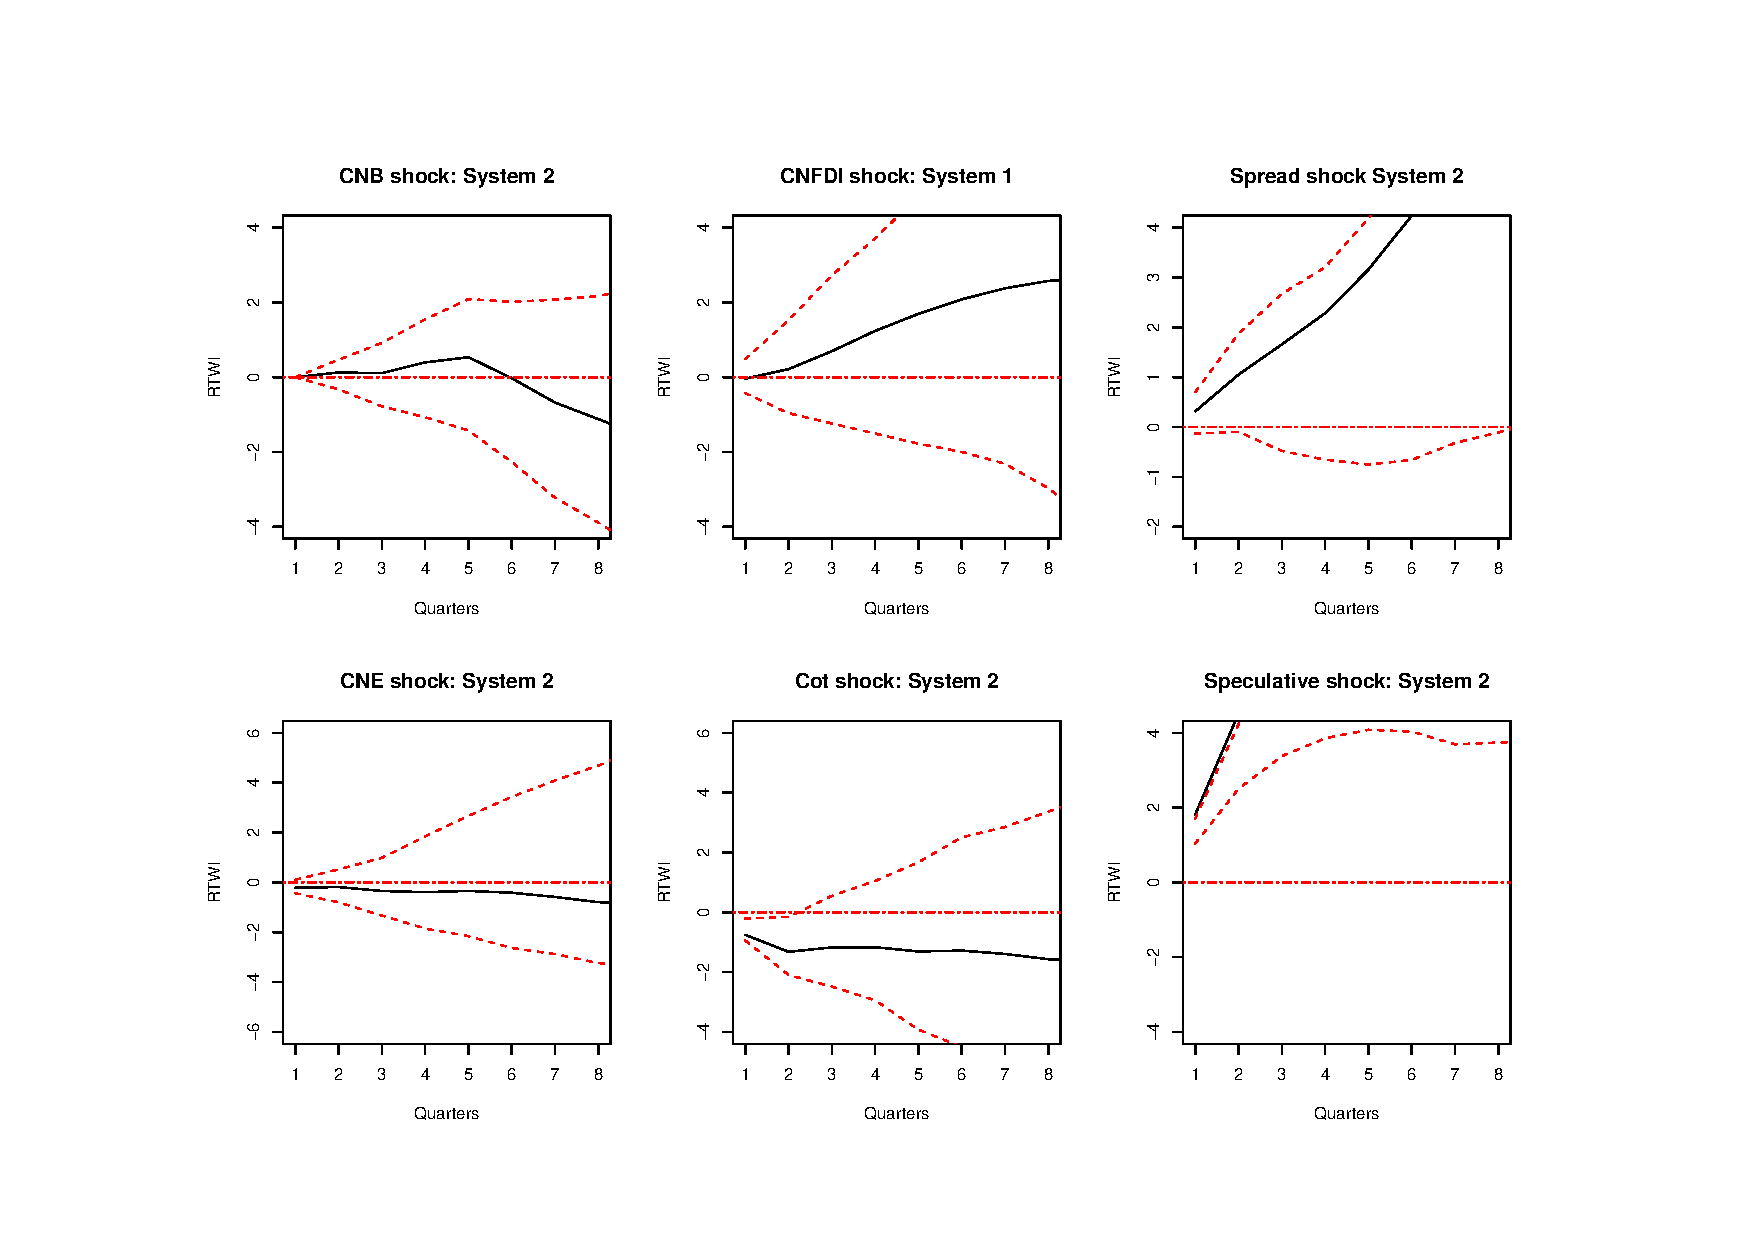
\includegraphics[scale=0.8]{IRF2}
\end{figure}
\end{landscape} 


\section{Speculation has real and significant effects} 
A model of international capital flow and the real exchange rate has been presented.  A VAR has been used to estimate the parameters of the system, using data that has been collected from a variety of sources, and these estimated parameters are used to create IRFs that show how the system returns to stability once it has been hit by a shock.  Unlike most attempts to assess the relationship between capital flow and the exchange rate, this model includes a role for speculation, and some methods have been proposed here to measure speculative activity.  These measures seek to capture two types of speculative activity:  sentiment driven and interest rate driven.  

The IRFs that have been presented suggest that deviations from PPP can be explained by innovations in net international capital flows and that, contrary to some of the other investigations of this issue, the type of flow that has the most pronounced and significant effect is that associated with speculation.  If the assumption is made that PPP is the fundamental value, this means that speculation is the key factor that is driving the exchange rate away from equilibrium.  However, the nature of the method used here, derived from the microstructure literature and focused on orders, means that the underlying motivation of the financial flows is not known.  It is  assumed to include any of those factors that have been left out of the model in the pursuit of parsimony.  The reason that speculators become more positive about the US dollar is not known.  It may be benign, part of the process of price adjustment, with changes in the underlying fundamentals requiring a need for a change in the real exchange rate (as was discussed in Section \ref{secref:HBS}), it may be that these changes in the real exchange rate are not justified by economic fundamentals and the speculative activity is upsetting the equilibrium and causing an imbalance. 

The type of information that is behind the speculative activity is important.  If speculation is informed, it is part of the process of \emph{price discovery}, it is an important part of ensuring that exchange rates reflect economic fundamentals, and it speeds the process that aligns prices with fundamentals; if speculation is uninformed, it is distorting prices and providing false signals.  Looking at Figure \ref{fig:timeseries} it is clear from the time series graph of the real exchange rate (RTWI in row 2, column 2 of the figure) that there have been some substantial changes in the value of the US real exchange rate.  The very large appreciation that is evident in the period between 2000 and 2005 may have been a reaction to fundamentals.  It is not possible to determine that from the methods used in this chapter.  

The appreciation of the US real exchange rate may be the cause of a number of significant US economic problems:  the deindustrialisation of the US economy, the problems faced by the auto industry and increase in economic inequality.  The rise in the US current account deficit has been part of the story of global imbalances and consequent increase in international capital flows contributing, in some eyes, to the  sub-prime crisis and financial shock (see Footnote \ref{note1} for detail).  As such, an investigation of the informational content of speculation is of major importance.  

The next two chapters will explore speculation in more detail.  Chapter \ref{Chapter3} will assess the informational content of speculation with an assessment of speculative sentiment and momentum trading. This is the sort of activity that variable S1 is designed to capture in the capital flow system.  Chapter \ref{Chapter4} will look in detail at speculative activity that is associated with the \emph{carry trade} and will seek to understand more about the sort of returns that are achieved by that action. 


\bibliography{../../../../myrefs}

\begin{appendices}

\end{appendices}

\end{document}
